\documentclass[a4paper,12pt]{article}
\usepackage[russian]{babel}

% Самые необходимые пакеты
\usepackage[T2A]{fontenc}
\usepackage[utf8]{inputenc}
\usepackage[russian]{babel}
\usepackage{geometry}
\usepackage{amsmath}
\usepackage{graphicx}
\usepackage{float} 
\usepackage{xcolor}
\usepackage{listings}
\usepackage{hyperref}
\usepackage{array}
\usepackage{caption}
\usepackage{booktabs}
\usepackage{amssymb}
\usepackage{subcaption}
\usepackage{caption}
\captionsetup[figure]{name=Рисунок}
\captionsetup[table]{name=Таблица}
\usepackage{pgfplots}
\pgfplotsset{compat=1.18}
\usetikzlibrary{arrows.meta}
\usepackage{capt-of}
\usepackage{multirow}
\usepackage[siunitx]{circuitikz}
\usepackage[bottom]{footmisc}
\usepackage{tcolorbox}


\lstset{
	language=Matlab,
	basicstyle=\ttfamily\small,
	keywordstyle=\color{blue}\bfseries,
	commentstyle=\color{gray}\itshape,
	stringstyle=\color{red},
	numberstyle=\tiny\color{gray},
	numbers=left,
	stepnumber=1,
	numbersep=8pt,
	backgroundcolor=\color{white},
	frame=single,
	breaklines=true,
	breakatwhitespace=true,
	tabsize=4,
	showspaces=false,
	showstringspaces=false,
	captionpos=b,
	escapeinside={\%*}{*)},
}
\geometry{left=1.5cm, right=2cm, bottom=2cm, top=2cm}

\begin{document}
	
	% Титульный лист
	\begin{titlepage}
		\centering
		\vspace*{1cm}
		
		% Министерство
		{\small
			Министерство науки и высшего образования Российской Федерации\\
			Федеральное государственное автономное образовательное учреждение\\
			высшего образования\\
			«Национальный исследовательский университет ИТМО»\\
		}
		
		\vspace{2cm}
		
		% Факультет
		{\large
			Факультет систем управления и робототехники\\
		}
		
		\vspace{3cm}
		
		% Основной заголовок
		{\Huge\bfseries
			ОТЧЕТ\\
		}
		\vspace{0.5cm}
		{\LARGE\bfseries
			о лабораторной работе №6\\
		}
		
		\vspace{1cm}
		
		% Дисциплина и тема
		{\Large
			По дисциплине: «Линейные системы автоматического управления»\\
			\vspace{0.5cm}
			Тема: «Критерий Найквиста и системы с запаздыванием»\\
		}
		
		\vspace{3cm}
		
		% Информация о студенте и преподавателях
		\begin{minipage}{0.4\textwidth}
			\raggedright
			{\large
				Студент:\\
			}
			Охрименко Е. Д.\\
			Поток: 1.1.3\\
			Вариант: 17\\
		\end{minipage}
		\hfill
		\begin{minipage}{0.4\textwidth}
			\raggedleft
			{\large
				Преподаватель:\\
			}
			Пашенко А. В.\\
		\end{minipage}
		
		\vfill
		
		% Город и год
		{\large
			Санкт-Петербург\\
			2026\\
		}
		
	\end{titlepage}
	
	\newpage
	\tableofcontents
	
	
	\newpage
	\section{Годограф Найквиста}
	
	В соответствии с моим вариантом рассмотрю три объекта пятого порядка \(5\) полюсов передаточных функций которых вещественные, а \(0\) -- комплексно-сопряженные.
	
	\begin{itemize}
		\item Передаточная функция 1 имеет \(3\) неустойчивых полюсов у разомкнутой системы и \(2\) неустойчивых полюсов у замкнутой.
		
		\item Передаточная функция 2 имеет \(0\) неустойчивых полюсов у разомкнутой системы и \(2\) неустойчивых полюсов у замкнутой.
		
		\item Передаточная функция 3 имеет \(3\) неустойчивых полюсов у разомкнутой системы и \(0\) неустойчивых полюсов у замкнутой.
		
	\end{itemize}
	
	
		Требуется:
	
	\begin{itemize}
		\item Построить карты нулей и полюсов разомкнутой и замкнутой систем на комплексной плоскости.
		
		\item Выполнить моделирование и получить переходные характеристики разомкнутой и замкнутой систем.
		
		\item Построить годограф Найквиста (АФЧХ), определить число его обходов вокруг точки $(-1;0)$ и сравнить результаты по критерию Найквиста.
		
		\item Построить ЛАЧХ и ЛФЧХ разомкнутой системы, определить число переходов ЛФЧХ через критические отрезки при положительной ЛАЧХ и проанализировать устойчивость по логарифмическому критерию Найквиста.
	\end{itemize}
	
	\hrule

	\newpage
	\subsection{Объект 1}
	
	Согласно моему варианту, требуется, чтобы полюса передаточной функции были вещественными.
	
	Запишу разомкнутую передаточную функцию, как отношение полинома числителя к полиному знаменателя:
	
	\[W_\text{раз}(s) = \frac{R(s)}{Q(s)}\]
	
	Запишу замкнутую передаточную функцию: \[W_\text{замк}(s) = \frac{W_\text{раз}(s)}{1 + W_\text{раз}(s)} = \frac{R(s) / Q(s)}{1 + R(s) / Q(s)} = \frac{R(s)}{R(s) + Q(s)}\]
	
	Пусть: \[Q'(s) = R(s) + Q(s) \quad \Longrightarrow \quad R(s) = Q'(s) - Q(s)\]
	
	Мне нужно иметь 3 неустойчивых полюса в разомкнутой системе. Выберу:
	
	\[Q(s) = (s-1)(s-2)(s-3)(s+4)(s+5)\]
	
	Раскрыв скобки, получу:
	
	\[Q(s) = s^5 + 3s^4 - 23s^3 - 27s^2 + 166s - 120\]
	
	Также нужно иметь 2 неустойчивых полюса в замкнутой системе. Выберу: 
	
	\[Q'(s) = (s+1)(s+2)(s+3)(s-6)(s-7)\]
	
	Раскрыв скобки, получу:
	
	\[Q'(s) = s^5 - 7s^4 - 25s^3 + 115s^2 + 384s + 252\]
	
	Теперь найду подходящий числитель:
	
	\begin{align*}
		R(s) 
		&= (s^5 - 7s^4 - 25s^3 + 115s^2 + 384s + 252) - (s^5 + 3s^4 - 23s^3 - 27s^2 + 166s - 120) \\
		&= (1-1)s^5 + (-7-3)s^4 + (-25+23)s^3 + (115+27)s^2 + (384-166)s + (252+120) \\
		&= -10s^4 - 2s^3 + 142s^2 + 218s + 372
	\end{align*}
	
	И наконец, запишу полученные передаточные функции:
	
	\[W_\text{раз}(s) = \frac{-10s^4 - 2s^3 + 142s^2 + 218s + 372}{(s-1)(s-2)(s-3)(s+4)(s+5)} \qquad W_\text{замк}(s) = \frac{-10s^4 - 2s^3 + 142s^2 + 218s + 372}{(s+1)(s+2)(s+3)(s-6)(s-7)}\]

	
	\newpage
	\subsubsection{Нули и полюса разомкнутой и замкнутой систем}
	
	Изображу карту нулей и полюсов разомкнутой и замкнутой систем на комплексной плоскости.
	
	\begin{figure}[H]
		\centering
		
		\newcommand{\w}{0.49\textwidth}
		
		\begin{minipage}{\w}
			\centering
			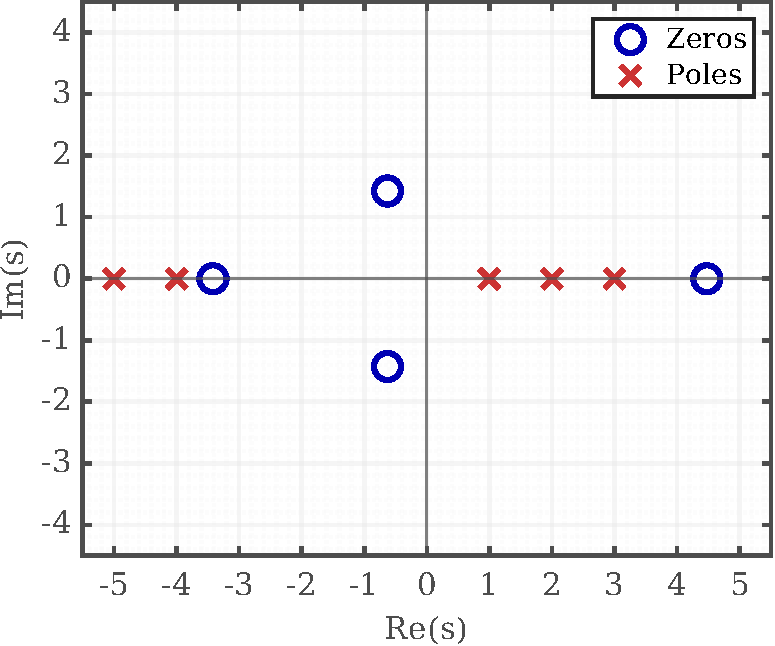
\includegraphics[width=\textwidth]{../images/task1/o1/PZ-plot-raz.pdf}
			\caption{Разомкнутая система}
		\end{minipage}
		\hfill
		\begin{minipage}{\w}
			\centering
			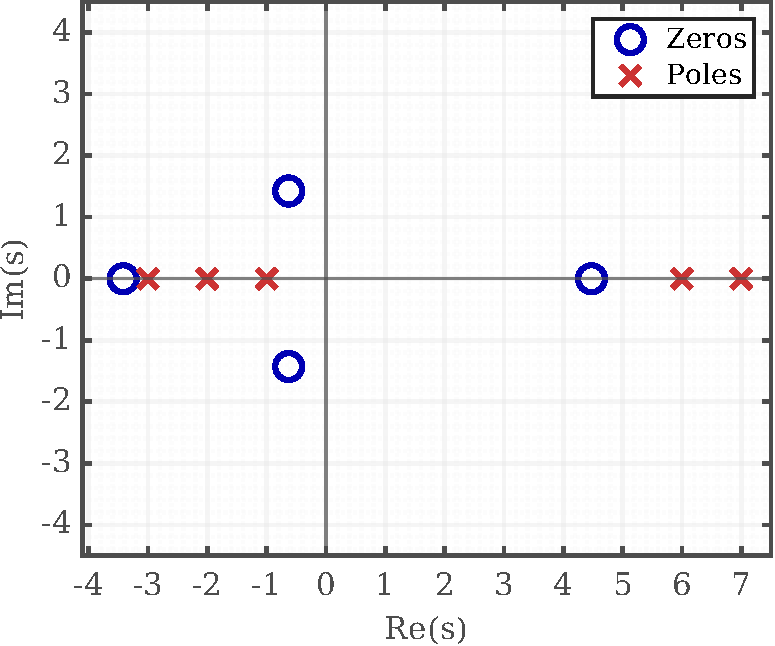
\includegraphics[width=\textwidth]{../images/task1/o1/PZ-plot-zamk.pdf}
			\caption{Замкнутая система}
		\end{minipage}
		
	\end{figure}
	
	Расположение полюсов сопоставляется с заявленным по заданию, в случае разомкнутой системы имею \(3\) неустойчивых полюса, в случае замкнутой \(2\). 
	
	\subsubsection{Переходные характеристики}
	
	Поскольку в обеих системах у меня есть неустойчивые полюса, то отклик систем на единичное ступенчатое воздействие будет возрастать:
	
	\[\lim_{t \to + \infty} y_{s.r}(t) = + \infty\]
	
	\begin{figure}[H]
		\centering
		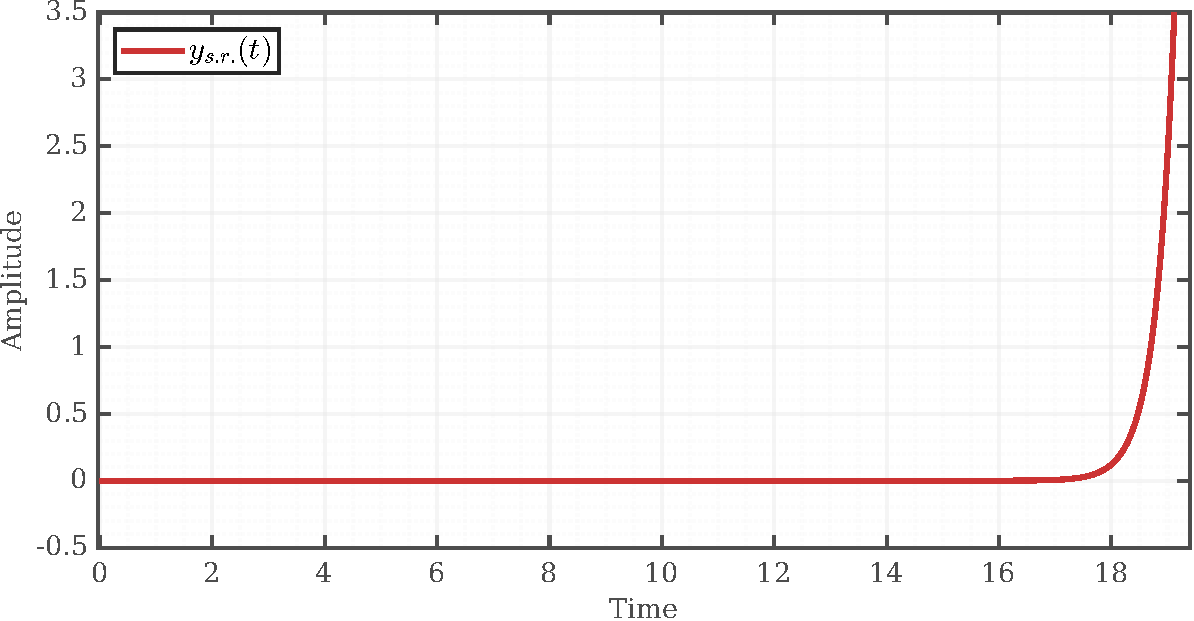
\includegraphics[width=1\textwidth]{../images/task1/o1/h-raz.pdf}
		\caption{Step Response разомкнутой системы}
	\end{figure}
	
	\begin{figure}[H]
		\centering
		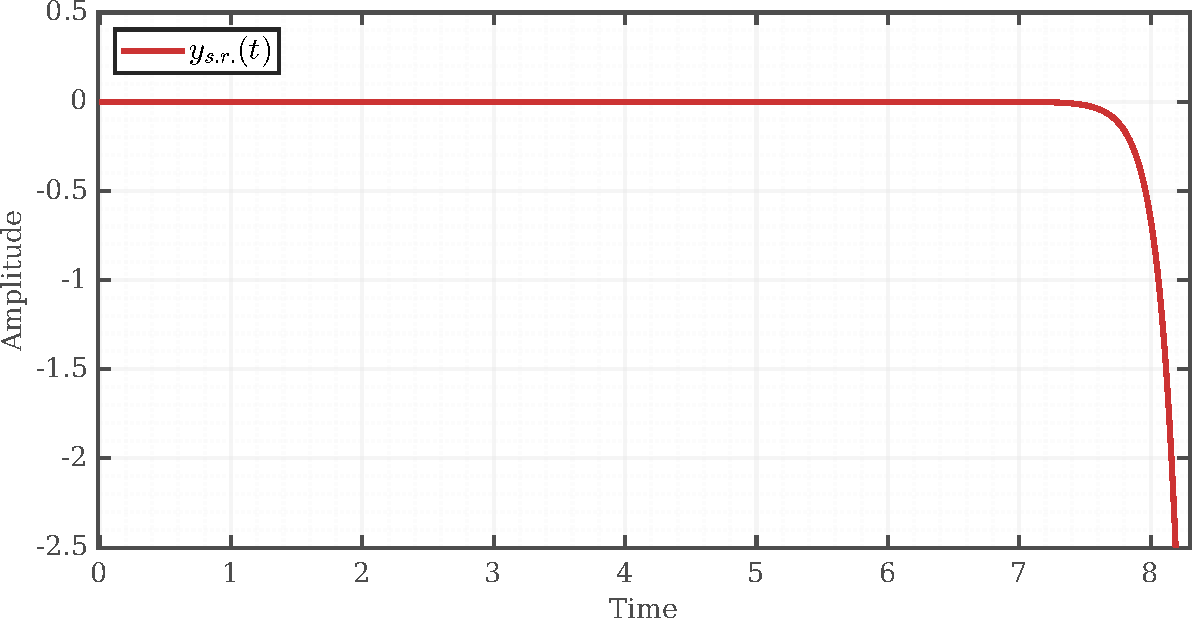
\includegraphics[width=1\textwidth]{../images/task1/o1/h-zamk.pdf}
		\caption{Step Response замкнутой системы}
	\end{figure}
	
	\subsubsection{Годограф Найквиста (АФЧХ)}
	
	
	\begin{figure}[H]
		\centering
		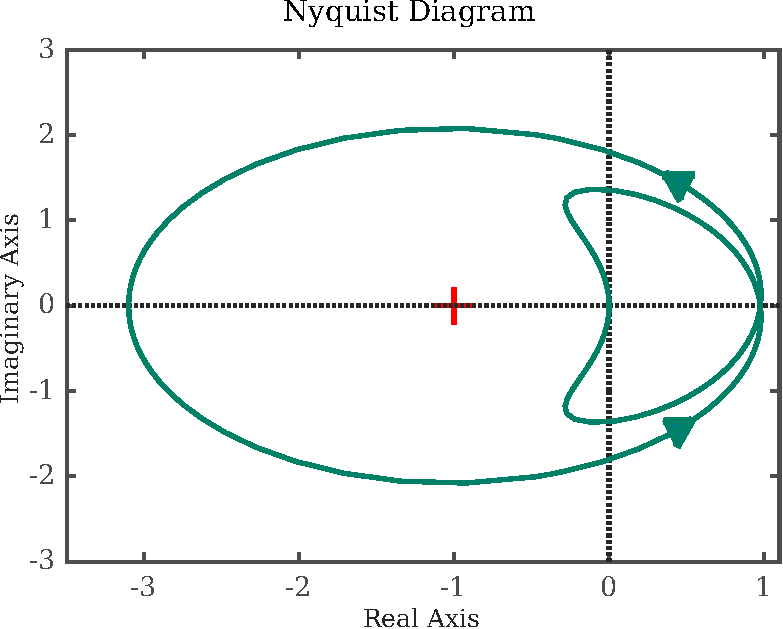
\includegraphics[width=0.65\textwidth]{../images/task1/o1/GNA.pdf}
		\caption{Годограф Найквиста}
	\end{figure}
	
	
	По годографу виден один обход против часовой стрелки, значит число оборотов вокруг точки \(-1; 0\) по часовой стрелке равняется \(-1\). 
	
	\[X = -1\]
	
	Применю критерий Найквиста: Число неустойчивых полюсов \(W_\text{раз}(s)\) + число оборотов годографа по часовой стрелке = число неустойчивых полюсов \(W_\text{замк}(s)\):
	
	\[n + X = m \quad \Longrightarrow \quad 3 - 1 = 2\]
	
	Равенство выполняется, число оборотов годографа по часовой стрелке вокруг точки \((-1; 0)\) и через критерий Найквиста эквивалентны.
	
	\subsubsection{ЛАЧХ и ЛФЧХ}
	
	
	\begin{figure}[H]
		\centering
		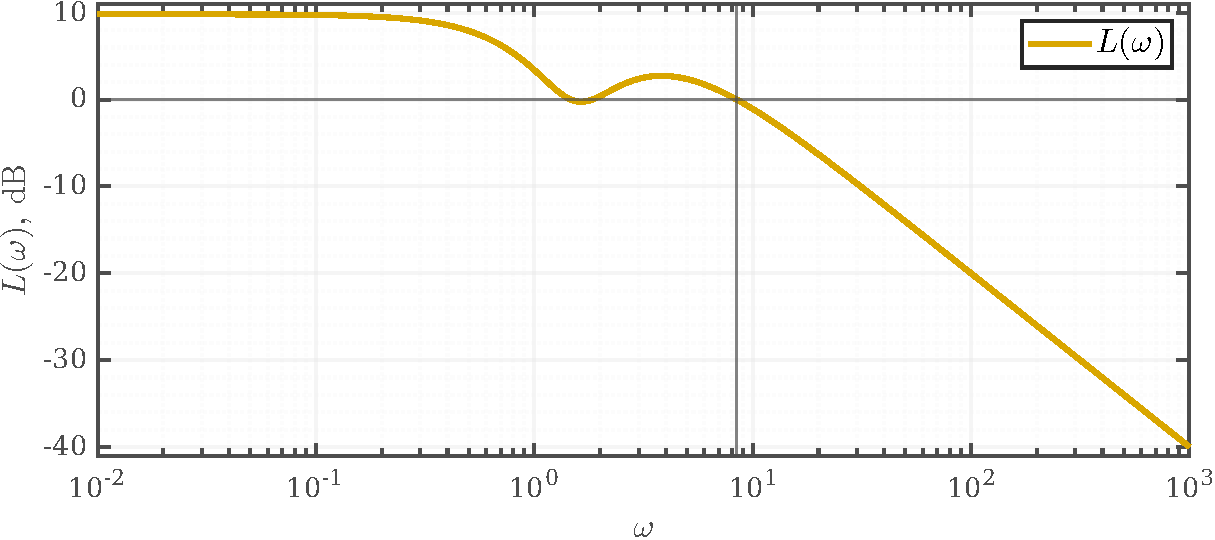
\includegraphics[width=0.9\textwidth]{../images/task1/o1/lach.pdf}
		\caption{ЛАЧХ разомкнутой системы}
	\end{figure}
	
	\begin{figure}[H]
		\centering
		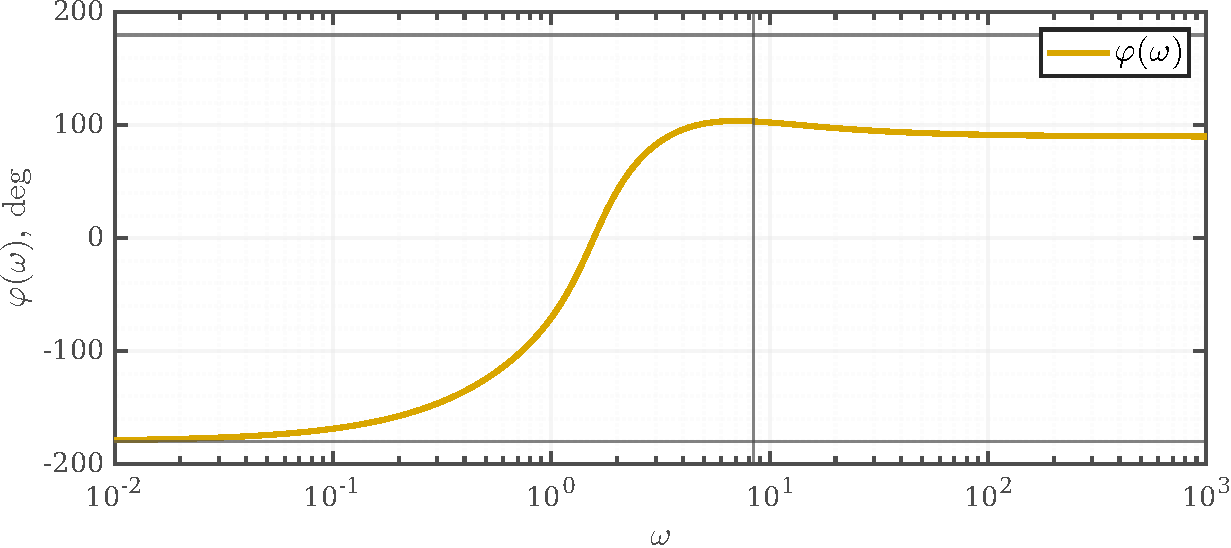
\includegraphics[width=0.9\textwidth]{../images/task1/o1/lfch.pdf}
		\caption{ЛФЧХ разомкнутой системы}
	\end{figure}
	
	Применю логарифмический критерий Найквиста.	Определю суммарное число переходов ЛФЧХ через уровни
	$\varphi(\omega)=(2k+1)\pi$ на частотах, где $L(\omega)>0$,
	учитывая их знак (положительные и отрицательные).
	Затем проверю соотношение:
	\[
	N = n/2
	\]
	где $n$ — число правых полюсов разомкнутой системы,
	$N$ — сумма переходов. Если равенство выполнено, система устойчива.
	
	ЛФЧХ не пересекает критические уровни, так как вся она расположена в диапазоне \([-\pi; \pi]\). Однако линия начинается с критического уровня и далее идет снизу вверх, значит:\[N = 0.5\]
	
	Так как равенство не выполняется:
	\[N = n/2 \quad \Longrightarrow \quad 0.5 \neq \frac{3}{2}\]
	
	
	логарифмический критерий Найквиста не выполнен, следовательно, замкнутая система не устойчива.
	
	Полученное значение совпадает с числом оборотов годографа Найквиста:
	\[
	2N = 1
	\]
	что соответствует одному обходу точки $(-1,0)$,
	найденным в предыдущем пункте.
	
	
	
	
	
	
	
	
	
    \newpage
	\subsection{Объект 2}
	
	Запишу разомкнутую передаточную функцию, как отношение полинома числителя к полиному знаменателя:
	
	\[W_\text{раз}(s) = \frac{R(s)}{Q(s)}\]
	
	Запишу замкнутую передаточную функцию: \[W_\text{замк}(s) = \frac{W_\text{раз}(s)}{1 + W_\text{раз}(s)} = \frac{R(s) / Q(s)}{1 + R(s) / Q(s)} = \frac{R(s)}{R(s) + Q(s)}\]
	
	Пусть: \[Q'(s) = R(s) + Q(s) \quad \Longrightarrow \quad R(s) = Q'(s) - Q(s)\]
	
	Мне нужно иметь \(0\) неустойчивых вещественных полюсов в разомкнутой системе. Выберу:
	
	\[Q(s) = (s+1)(s+2)(s+3)(s+4)(s+5)\]
	
	Раскрыв скобки, получу:
	
	\[Q(s) = s^5 + 15s^4 + 85s^3 + 225s^2 + 274s + 120\]
	
	Также нужно иметь 2 неустойчивых вещественных полюса в замкнутой системе. Выберу: 
	
	\[Q'(s) = (s-1)(s-2)(s+6)(s+7)(s+8)\]
	
	Раскрыв скобки, получу:
	
	\[Q'(s) = s^5 + 18s^4 + 85s^3 - 60s^2 - 716s + 672\]
	
	Теперь найду подходящий числитель:
	
	\begin{align*}
		R(s) 
		&= (s^5 + 18s^4 + 85s^3 - 60s^2 - 716s + 672) - (s^5 + 15s^4 + 85s^3 + 225s^2 + 274s + 120) \\
		&= (1-1)s^5 + (18-15)s^4 + (85-85)s^3 + (-60-225)s^2 + (-716-274)s + (672-120) \\
		&= 3s^4 - 285s^2 - 990s + 552
	\end{align*}
	
	И наконец, запишу полученные передаточные функции:
	
	\[W_\text{раз}(s) = \frac{3s^4 - 285s^2 - 990s + 552}{(s+1)(s+2)(s+3)(s+4)(s+5)} \qquad W_\text{замк}(s) = \frac{3s^4 - 285s^2 - 990s + 552}{(s-1)(s-2)(s+6)(s+7)(s+8)}\]
	
	\newpage
	\subsubsection{Нули и полюса разомкнутой и замкнутой систем}
	
	У разомкнутой системы все полюса лежат строго в левой комплексной полуплоскости, а у замкнутой имею 2 неустойчивых и 3 устойчивых полюса.
	
		\begin{figure}[H]
		\centering
		
		\newcommand{\w}{0.49\textwidth}
		
		\begin{minipage}{\w}
			\centering
			
\includegraphics[width=\textwidth]{../images/task1/o2/PZ-plot-raz.pdf}
			\caption{Разомкнутая система}
		\end{minipage}
		\hfill
		\begin{minipage}{\w}
			\centering
			
\includegraphics[width=\textwidth]{../images/task1/o2/PZ-plot-zamk.pdf}
			\caption{Замкнутая система}
		\end{minipage}
		
	\end{figure}
	
	\subsubsection{Переходные характеристики}
	
	Поскольку полюса \(W_\text{раз}(s)\) лежат в левой комплексной полуплоскости, то \(y_{s.r}(t)\) разомкнутой системы будет ограничен.
	
	\begin{figure}[H]
		\centering
		
\includegraphics[width=1\textwidth]{../images/task1/o2/h-raz.pdf}
		\caption{Step Response разомкнутой системы}
	\end{figure}
	
	\newpage
	А у замкнутой системы есть неустойчивые полюса, значит:
	
	\[\lim_{t \to + \infty} y_{s.r}(t) = + \infty\]
	
	\begin{figure}[H]
		\centering
		
\includegraphics[width=1\textwidth]{../images/task1/o2/h-zamk.pdf}
		\caption{Step Response замкнутой системы}
	\end{figure}
	
	\subsubsection{Годограф Найквиста (АФЧХ)}	
	 
	\begin{figure}[H]
		\centering
		
\includegraphics[width=0.65\textwidth]{../images/task1/o2/GNA.pdf}
		\caption{Годограф Найквиста}
	\end{figure}
	
	\newpage
	Число оборотов по часовой стрелке вокруг красной точки \((-1; 0)\) соответствует двум:
	
	\[X = 2\]
	
	Посчитаю число обходов  (\(Z\)) годографа вокруг \((-1; 0)\) при помощи критерия Найквиста:
	
	\[Z = m - n, \quad  m = 2, n = 0 \quad \Longrightarrow \quad Z = 2\]
	
	Так как \(X=Z\), критерий выполнен, количество оборотов, найденных графически и аналитически совпадают.
	
	\subsubsection{ЛАЧХ и ЛФЧХ}
	
	\begin{figure}[H]
		\centering
		
\includegraphics[width=0.9\textwidth]{../images/task1/o2/lach.pdf}
		\caption{ЛАЧХ разомкнутой системы}
	\end{figure}
	
	\begin{figure}[H]
		\centering
		
\includegraphics[width=0.9\textwidth]{../images/task1/o2/lfch.pdf}
		\caption{ЛФЧХ разомкнутой системы}
	\end{figure}
	
	Применю логарифмический критерий Найквиста.	Определю суммарное число переходов ЛФЧХ через уровни
	$\varphi(\omega)=(2k+1)\pi$ на частотах, где $L(\omega)>0$,
	учитывая их знак (положительные и отрицательные).
	Затем проверю соотношение:
	\[
	N = n/2
	\]
	где $n$ — число правых полюсов разомкнутой системы,
	$N$ — сумма переходов. Если равенство выполнено, система устойчива.
	
	На участке, где $L(\omega)>0$, ЛФЧХ пересекает уровень
	$\varphi(\omega)=\pi$ один раз сверху вниз,
	что соответствует одному отрицательному переходу. А поскольку ЛФЧХ не начинается на критическом отрезке, дополнительный переход учитывать не нужно.	\[N = -1\]

	
	Так как равенство не выполняется:
	\[N = n/2 \quad \Longrightarrow \quad -1 \neq \frac{0}{2}\]
	
	
	логарифмический критерий Найквиста не выполнен, следовательно, замкнутая система не устойчива.
	
	Полученное значение совпадает с числом оборотов годографа Найквиста:
	\[
	2N = -2
	\]
	что соответствует двум обходам точки $(-1,0)$,
	найденным в предыдущем пункте.
	
	
	\newpage
	\subsection{Объект 3}
	
	Запишу разомкнутую передаточную функцию, как отношение полинома числителя к полиному знаменателя:
	
	\[W_\text{раз}(s) = \frac{R(s)}{Q(s)}\]
	
	Запишу замкнутую передаточную функцию: \[W_\text{замк}(s) = \frac{W_\text{раз}(s)}{1 + W_\text{раз}(s)} = \frac{R(s) / Q(s)}{1 + R(s) / Q(s)} = \frac{R(s)}{R(s) + Q(s)}\]
	
	Пусть: \[Q'(s) = R(s) + Q(s) \quad \Longrightarrow \quad R(s) = Q'(s) - Q(s)\]
	
	Мне нужно иметь \(3\) неустойчивых вещественных полюса в разомкнутой системе. Выберу:
	
	\[Q(s) = (s-1)(s-2)(s-3)(s+4)(s+5)\]
	
	Раскрыв скобки, получу:
	
	\[Q(s)=s^5+3s^4-23s^3-27s^2+166s-120\]
	
	Также нужно иметь 0 неустойчивых вещественных полюсов в замкнутой системе. Выберу: 
	
	\[Q'(s) = (s+1)(s+2)(s+3)(s+6)(s+7)\]
	
	Раскрыв скобки, получу:
	
	\[Q'(s) = s^5+19s^4+131s^3+401s^2+540s+252\]
	
	Теперь найду подходящий числитель:

	\begin{align*}
		R(s) 
		&= (s^5+19s^4+131s^3+401s^2+540s+252) - (s^5+3s^4-23s^3-27s^2+166s-120) \\
		&= (1-1)s^5 + (19-3)s^4 + (131+23)s^3 + (401+27)s^2 + (540-166)s + (252+120) \\
		&= 16s^4 + 154s^3 + 428s^2 + 374s + 372
	\end{align*}
	
	И наконец, запишу полученные передаточные функции:
	
	\[W_\text{раз}(s) = \frac{16s^4 + 154s^3 + 428s^2 + 374s + 372}{(s-1)(s-2)(s-3)(s+4)(s+5)} \qquad W_\text{замк}(s) = \frac{16s^4 + 154s^3 + 428s^2 + 374s + 372}{(s+1)(s+2)(s+3)(s+6)(s+7)}\]
	
	
	\newpage
	\subsubsection{Нули и полюса разомкнутой и замкнутой систем}
	
	Количество неустойчивых полюсов разомкнутой системы соответствует \(3\), а замкнутая система имеет только устойчивые полюса.
	
	\begin{figure}[H]
		\centering
		
		\newcommand{\w}{0.49\textwidth}
		
		\begin{minipage}{\w}
			\centering
			
\includegraphics[width=\textwidth]{../images/task1/o3/PZ-plot-raz.pdf}
			\caption{Разомкнутая система}
		\end{minipage}
		\hfill
		\begin{minipage}{\w}
			\centering
			
\includegraphics[width=\textwidth]{../images/task1/o3/PZ-plot-zamk.pdf}
			\caption{Замкнутая система}
		\end{minipage}
		
	\end{figure}
	
	\subsubsection{Переходные характеристики}
	
	Поскольку у разомкнутой системы есть неустойчивые полюса, ее выход неограничен. 
	
	
	\begin{figure}[H]
		\centering
		
\includegraphics[width=1\textwidth]{../images/task1/o3/h-raz.pdf}
		\caption{Step Response разомкнутой системы}
	\end{figure}
	
	\newpage
	Замкнутая система будет устойчивой из-за отсутствия неустойчивых полюсов.

	\begin{figure}[H]
		\centering
		
\includegraphics[width=1\textwidth]{../images/task1/o3/h-zamk.pdf}
		\caption{Step Response замкнутой системы}
	\end{figure}
	

	\subsubsection{Годограф Найквиста (АФЧХ)}
	
	\begin{figure}[H]
		\centering
		
\includegraphics[width=0.65\textwidth]{../images/task1/o3/GNA.pdf}
		\caption{Годограф Найквиста}
	\end{figure}
	
	Число оборотов по часовой стрелке вокруг красной точки соответствует трём:
	
	\[X = -3\]
	
	Найду число обходов (\(Z\)) годографа вокруг \((-1; 0)\) при помощи критерия Найквиста:
	
	\[Z = m - n, \quad  m = 0, n = 3 \quad \Longrightarrow \quad Z = -3\]
	
	\(X=Z=-3\), что означает критерий выполнен, количество оборотов, найденных графически и аналитически совпадают.
	
	
	\subsubsection{ЛАЧХ и ЛФЧХ}
	
	\begin{figure}[H]
		\centering
		
\includegraphics[width=0.8\textwidth]{../images/task1/o3/lach.pdf}
		
		\vspace{0.5cm}
		
		
\includegraphics[width=0.8\textwidth]{../images/task1/o3/lfch.pdf}
		
		\caption{ЛАФЧХ разомкнутой системы}
	\end{figure}

	Применю логарифмический критерий Найквиста.	Определю суммарное число переходов ЛФЧХ через уровни
	$\varphi(\omega)=(2k+1)\pi$ на частотах, где $L(\omega)>0$,
	учитывая их знак (положительные и отрицательные).
	Затем проверю соотношение:
	\[
	N = n/2
	\]
	где $n$ — число правых полюсов разомкнутой системы,
	$N$ — сумма переходов. Если равенство выполнено, система устойчива.
	
	На участке, где $L(\omega)>0$, ЛФЧХ пересекает уровень
	$\varphi(\omega)=-\pi$ один раз снизу вверх,
	что соответствует одному положительному переходу. А поскольку ЛФЧХ начинается на критическом отрезке,
	дополнительно учитываю переход, равный $1/2$ с соответствующим положительным знаком:	
	\[
	N = 1 + \frac{1}{2} = 1.5
	\]
	
	Так как равенство выполняется:
	\[N = n/2 \quad \Longrightarrow \quad 1.5 = \frac{3}{2}\]
	
	
	логарифмический критерий Найквиста выполнен, следовательно, замкнутая система устойчива.
	
	Полученное значение совпадает с числом оборотов годографа Найквиста:
	\[
	2N = 3
	\]
	что соответствует трём обходам точки $(-1,0)$,
	найденным в предыдущем пункте.
	
	\newpage
	\subsection{Вывод по заданию}
	
	В этом задании я рассмотрела различные количества неустойчивых полюсов у разомкнутой и замкнутой систем. Построила их переходные характеристики, карты нулей и полюсов, годограф Найквиста и ЛАФЧХ. 
	
	Применила критерии Найквиста, проверила соотношение между ними. Получилось, что число оборотов годографа равняется числу переходов ЛФЧХ через критические уровни при положительной ЛАЧХ, умноженной на 2. Полученные результаты согласуются между собой и подтверждают сделанные выводы об устойчивости исследуемых замкнутых систем.

	
	
	
	
	
	
	
	
	
	
	
	
	
	
	
	
	
	
	
	
	\newpage
	\section{Коэффициент усиления}
	
	В соответствии с вариантом возьму значение \(i = 3\) и соответствующие ПФ:
	
	\[W_1(s) = \dfrac{s-4}{s^2 +8s + 2}\]
	
	\[W_2(s) = \dfrac{10s^2 + 9s - 1}{10s^3 - 12s^2 - s + 4}\]
	
	Добавлю к каждой функции коэффициент усиления: \[k > 0\]
		Требуется:
	
	\begin{itemize}
		\item Построить годограф Найквиста \((k = 1)\).
		
		\item Оценить влияние \(k_i\) на кривую годографа \( (i >= 3)\).
		
		\item Определить зависимость числа неустойчивых полюсов замкнутой системы от \(k\).
		
		\item Найти диапазон значений коэффициента усиления, при которых замкнутая система устойчива.
		
		\item Определить значение запаса устойчивости по амплитуде.
		
		\item Выполнить моделирование и привести переходные характеристики замкнутой системы.
	\end{itemize}
	
	
	\hrule
	
	
	
	
	\newpage
	\subsection{Объект 1}
	
	Первому объекту соответствует передаточная функция:
	
	\[W_1(s) = k \cdot \dfrac{s-4}{s^2 +8s + 2}\]
	
	\subsubsection{Математическая модель}
	
	Посчитаю \(W_\text{замк1}(s)\). Представлю \(W_1(s)\) как отношение полиномов:
	
	\[W_1(s) = \frac{k \cdot R(s)}{Q(s)}\]
	
	Запишу замкнутую передаточную функцию:
	
	 \[W_\text{замк1}(s) = \frac{W_1(s)}{1 + W_1(s)} = \frac{k \cdot R(s) / Q(s)}{1 + k \cdot R(s) / Q(s)} = \frac{k \cdot R(s)}{k \cdot R(s) + Q(s)}\]
	 
	 Тогда: 
	 
	 \[W_\text{замк1}(s) = \frac{k \cdot(s-4)}{s^2 + (k + 8)s + (-4k +2)}\]
	 
	 Теперь применю критерий Найквиста для анализа устойчивости системы. С помощью него найду пределы значений коэффициента усиления, относительно которых замкнутая система устойчива.
	 
	 Посчитаю количество неустойчивых полюсов разомкнутой системы:
	 
	 \[ s^2 +8s + 2 = 0
	 \quad \Longrightarrow \quad
	 s_{1,2} = -4 \pm \sqrt{14}	< 0  \]
	 
	 
	 Разомкнутая система имеет 2 устойчивых полюса и не имеет неустойчивых:
	 
	 \[n = 0\]

	\subsubsection{Влияние коэффициента усиления на кривую годографа}
	
	Построю годографы для следующих значений \(k\):
	
	\[
	\begin{cases}
		k_1 = \dfrac{1}{5} \\[8pt]
		k_2 = \dfrac{1}{2} \\[8pt]
		k_3 = \dfrac{3}{2} 
	\end{cases}
	\]
	
	А также построю годограф Найквиста при \(k = 1\).
	
	Заметно, что при увеличении \(k\) годограф начинает растягиваться относительно начала координат. А также количество оборотов увеличивается с нуля до одного.
	
	\begin{figure}[H]
		\centering
		
		\newcommand{\w}{0.49\textwidth}
		
		\begin{minipage}{\w}
			\centering
			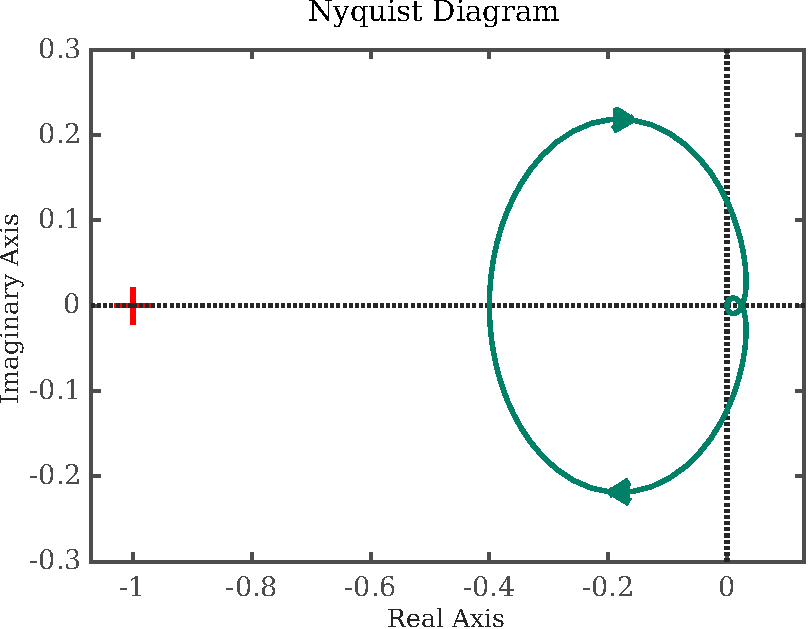
\includegraphics[width=\textwidth]{../images/task2/o1/GNA2.pdf}
			\caption{\(k_1 = \dfrac{1}{5}\)}
		\end{minipage}
		\hfill
		\begin{minipage}{\w}
			\centering
			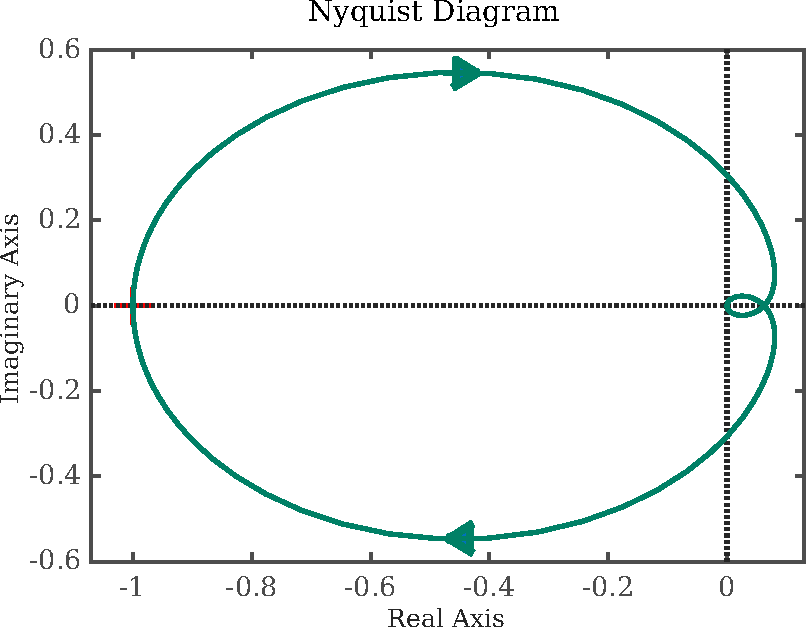
\includegraphics[width=\textwidth]{../images/task2/o1/GNA3.pdf}
			\caption{\(k_1 = \dfrac{1}{2}\)}
		\end{minipage}
		\hfill
		\\[15pt]
		\begin{minipage}{\w}
			\centering
			
\includegraphics[width=\textwidth]{../images/task2/o1/GNA.pdf}
			\caption{\(k_1 = 1\)}
		\end{minipage}
		\hfill
		\begin{minipage}{\w}
			\centering
			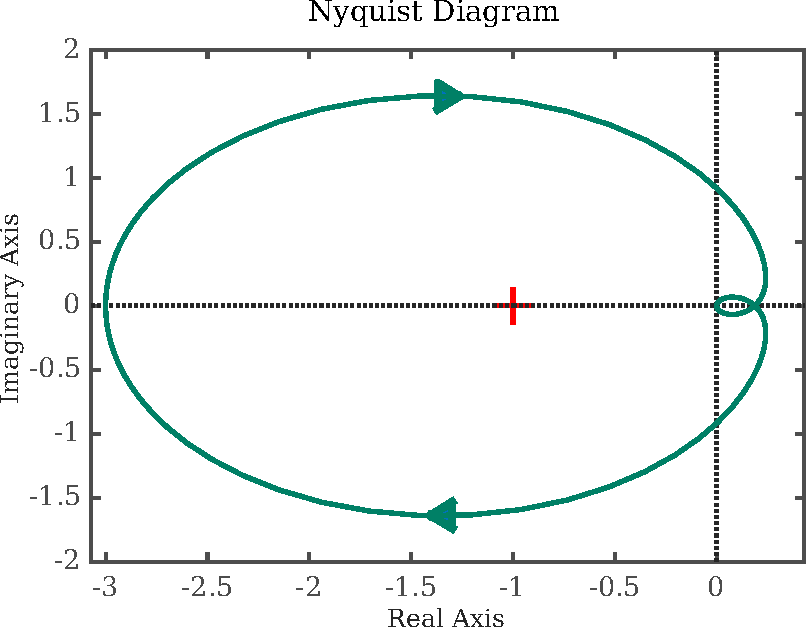
\includegraphics[width=\textwidth]{../images/task2/o1/GNA4.pdf}
			\caption{\(k_1 = \dfrac{3}{2}\)}
		\end{minipage}
		
		\caption*{Рисунки 21-24: Годографы Найквиста для различных \(k\)}
	\end{figure}
	
	При \(0 < k < 0.5\) годограф Найквиста не охватывает точку \((-1,0)\), следовательно, число оборотов:
	\[
	X = 0
	\]
	По критерию Найквиста, соотношение неустойчивых полюсов у замкнутой системы и у разомкнутой:
	\[
	m = n + X.
	\]
	Так как \(n = 0\):
	\[
	m = 0 \quad \Longrightarrow \quad \text{замкнутая система устойчива}
	\]\\
	
	При \(k = 0.5\) годограф проходит через точку \((-1,0)\), что соответствует границе устойчивости замкнутой системы.\\
	
	При \(k > 0.5\) годограф совершает один обход точки \((-1,0)\):
	\[
	X = 1
	\]
	Число неустойчивых полюсов замкнутой системы:
	\[
	m = n + X \quad \Longrightarrow \quad m = 0 + 1 = 1
	\]
	то есть замкнутая система имеет один неустойчивый полюс.


	
	

	\subsubsection{Переходные характеристики замкнутой системы}
	
	
		\begin{figure}[H]
		\centering
		
		\newcommand{\w}{0.49\textwidth}
		
		\begin{minipage}{\w}
			\centering
			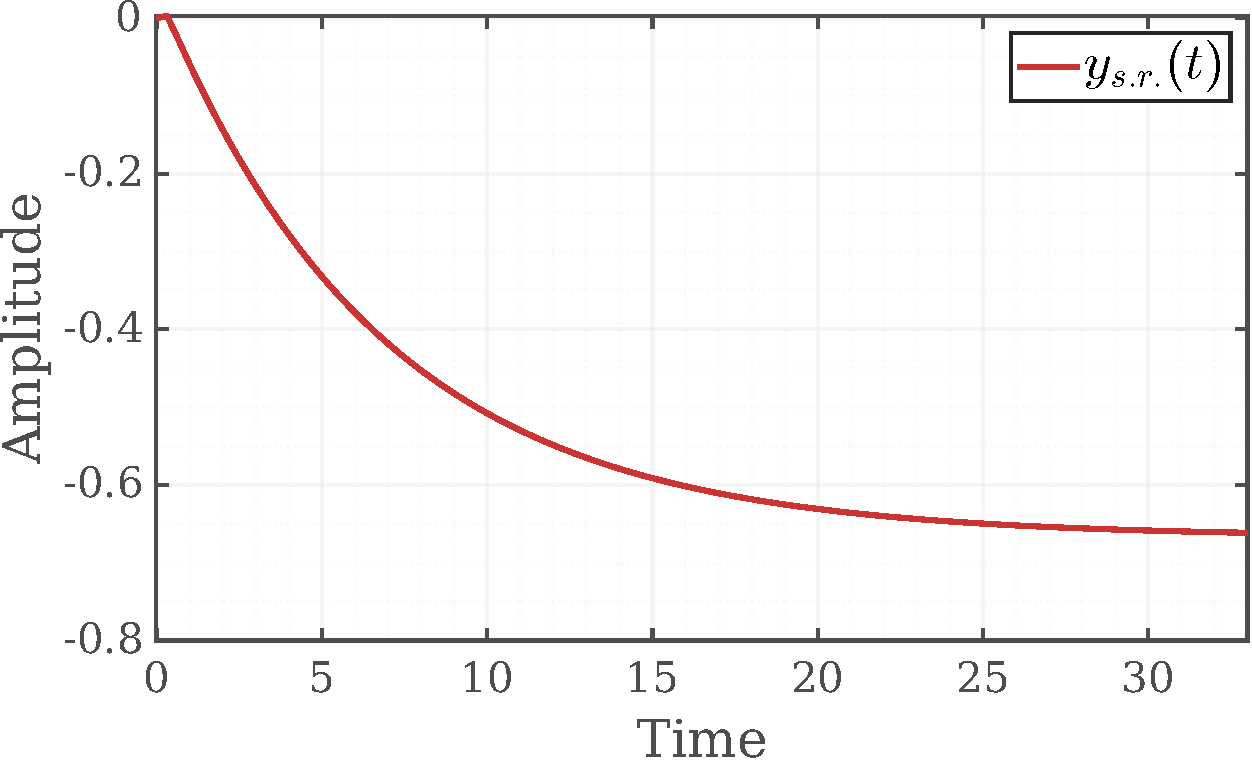
\includegraphics[width=\textwidth]{../images/task2/o1/h-zamk2.pdf}
			\caption{\(k_1 = \dfrac{1}{5}\)}
		\end{minipage}
		\hfill
		\begin{minipage}{\w}
			\centering
			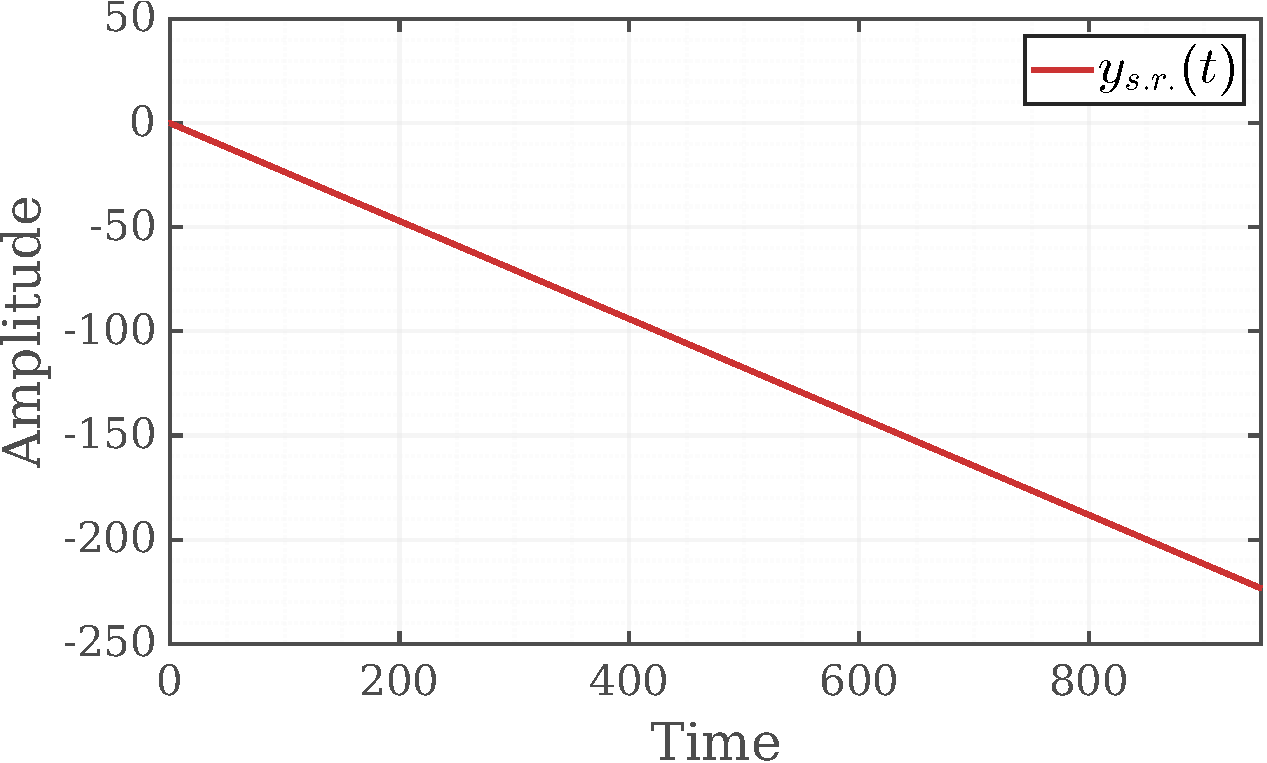
\includegraphics[width=\textwidth]{../images/task2/o1/h-zamk3.pdf}
			\caption{\(k_1 = \dfrac{1}{2}\)}
		\end{minipage}
		\hfill
		\\[15pt]
		\begin{minipage}{\w}
			\centering
			
\includegraphics[width=\textwidth]{../images/task2/o1/h-zamk.pdf}
			\caption{\(k_1 = 1\)}
		\end{minipage}
		\hfill
		\begin{minipage}{\w}
			\centering
			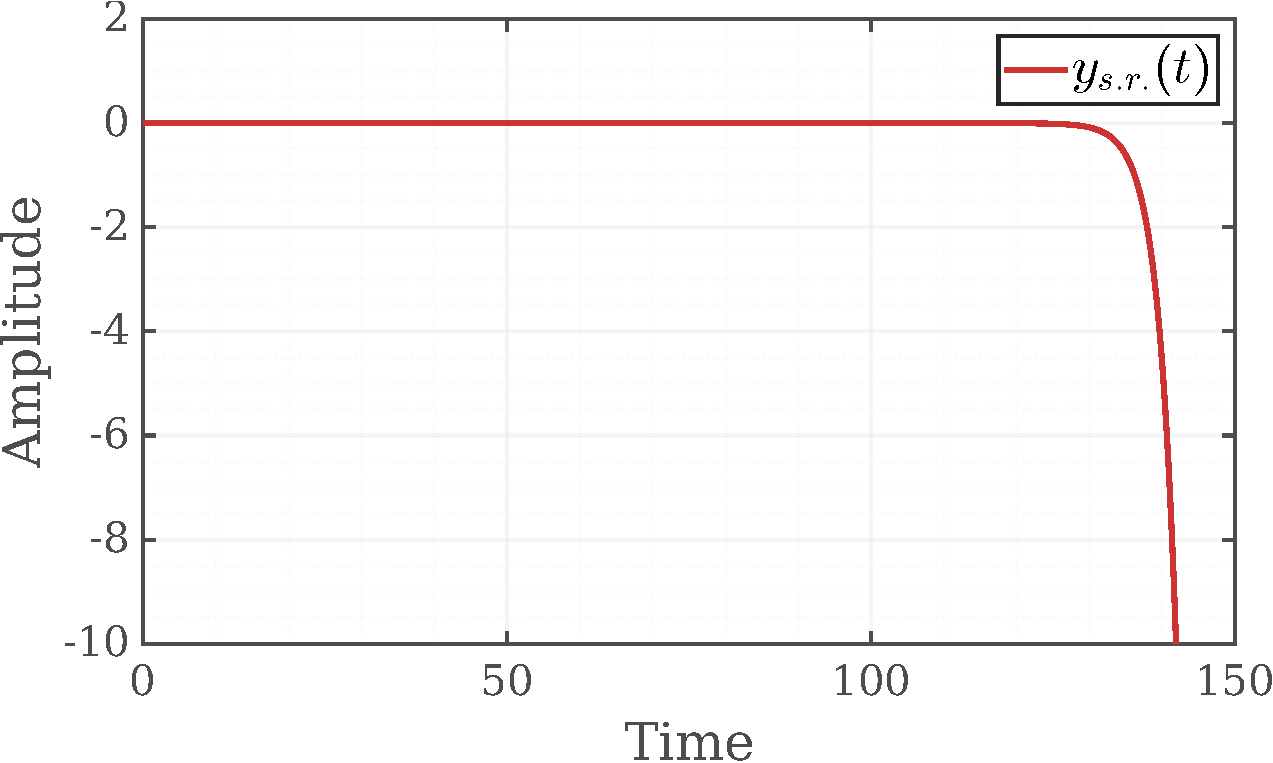
\includegraphics[width=\textwidth]{../images/task2/o1/h-zamk4.pdf}
			\caption{\(k_1 = \dfrac{3}{2}\)}
		\end{minipage}
		
		\caption*{Рисунки 25-28: Step Response замкнутых систем для различных \(k\)}
	\end{figure}
	
	Соотношения из предыдущего пункта подтверждаются на переходных характеристиках замкнутой системы.
	
	При \(k = \dfrac{1}{5}\) замкнутая система устойчива.\\[4pt]
	
	При \(k = \dfrac{1}{2}\) замкнутая система нейтрально устойчива.\\[4pt]
	
	При \(k = 1\) и \(k = \dfrac{3}{2}\) замкнутая система неустойчива.\\[4pt]
	
	\subsubsection{Зависимость количества неустойчивых полюсов от \(k\)}
	
	Чтобы определить зависимость количества неустойчивых полюсов замкнутой системы относительно значений коэффициента усиления построю карты нулей и полюсов, с соответственными \(k\).
	
	
	\begin{figure}[H]
		\centering
		
		\newcommand{\w}{0.46\textwidth}
		
		\begin{minipage}{\w}
			\centering
			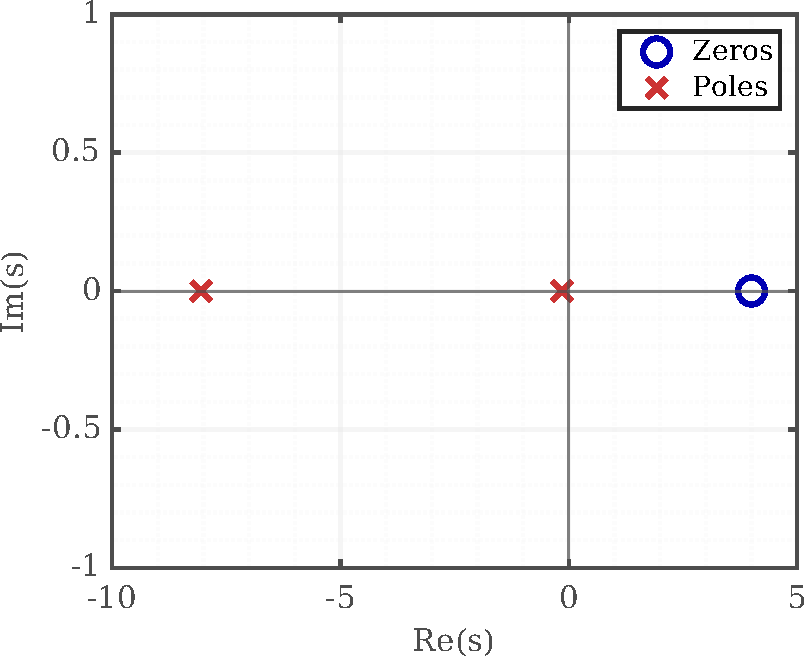
\includegraphics[width=\textwidth]{../images/task2/o1/PZ-plot2.pdf}
			\caption{\(k_1 = \dfrac{1}{5}\)}
		\end{minipage}
		\hfill
		\begin{minipage}{\w}
			\centering
			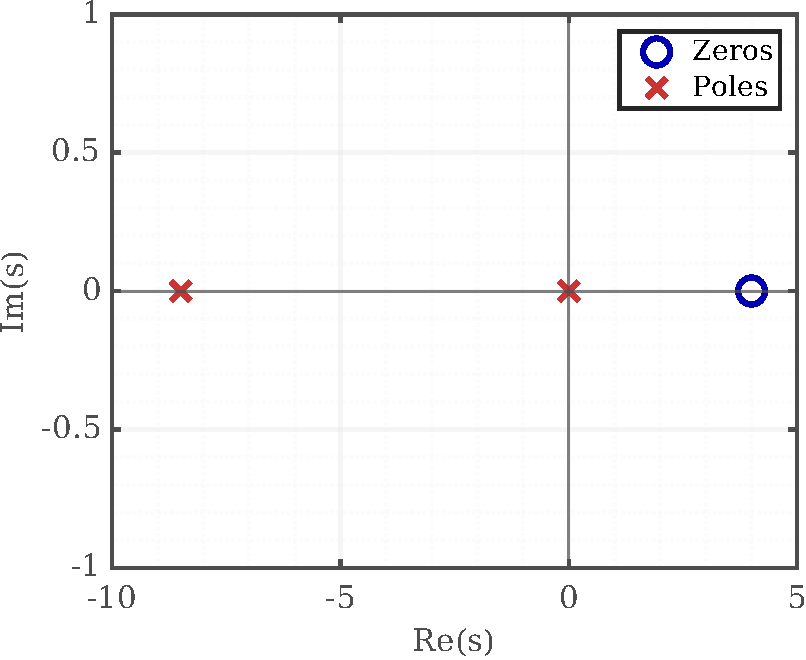
\includegraphics[width=\textwidth]{../images/task2/o1/PZ-plot3.pdf}
			\caption{\(k_1 = \dfrac{1}{2}\)}
		\end{minipage}
		\hfill
		\\[15pt]
		\begin{minipage}{\w}
			\centering
			
\includegraphics[width=\textwidth]{../images/task2/o1/PZ-plot.pdf}
			\caption{\(k_1 = 1\)}
		\end{minipage}
		\hfill
		\begin{minipage}{\w}
			\centering
			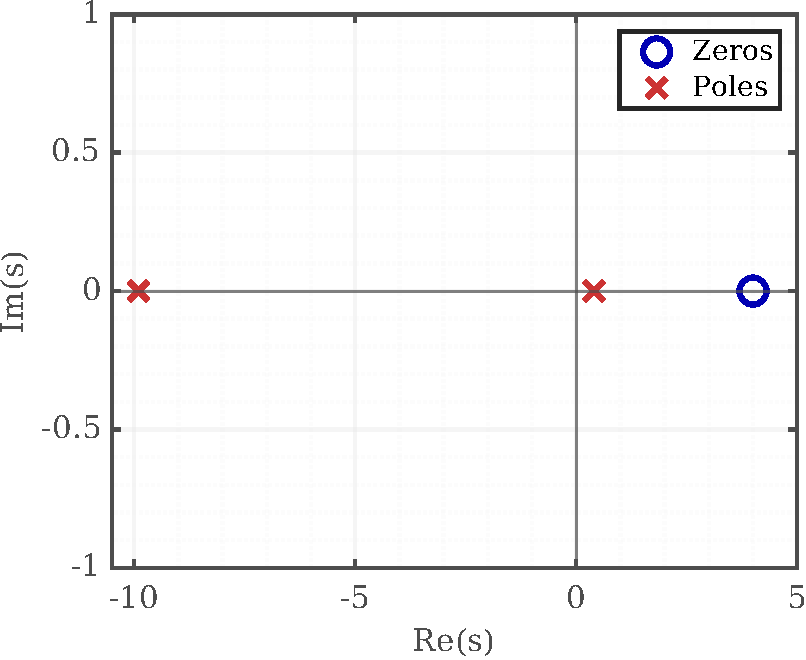
\includegraphics[width=\textwidth]{../images/task2/o1/PZ-plot4.pdf}
			\caption{\(k_1 = \dfrac{3}{2}\)}
		\end{minipage}
		
		\caption*{Рисунки 29-32: Карты нулей и полюсов замкнутых систем для различных \(k\)}
	\end{figure}	
	
	
	Замкнутая система имеет либо 0, либо 1 неустойчивый полюс.\\[4pt]
	
	Осталось рассмотреть случай, когда у системы может быть два неустойчивых полюса, и оценить, возможен ли он.
	
	Запишу характеристическое уравнение замкнутой системы:
	
	\[H(s) = s^2 + (k + 8)s + (-4k +2)\]
	
	Найду корни (полюса) по теореме Виета:
	
	\[
	\begin{cases}
		s_1 + s_2 = -(k+8) \\
		s_1 \cdot s_2 = 2-4k
	\end{cases}
	\]
	
	При этом, чтобы оба полюса были неустойчивыми должно выполняться условие: 
	
		\[
	\begin{cases}
		s_1 > 0 \\
		s_2 > 0
	\end{cases}
	\]
	
	Следовательно, их сумма и произведение должны быть положительными:
	
	\[
	\begin{cases}
		-(k+8) > 0\\
		2-4k > 0
	\end{cases}
	\qquad \Longrightarrow \qquad 
	\begin{cases}
		k < -8\\
		k < \dfrac{1}{2}
	\end{cases}
	\qquad \Longrightarrow \qquad 
	k < -8
	\]
	
	Но поскольку есть главное ограничение на положительность коэффициента \(k\) в условии задачи, случай, при котором замкнутая система имеет два неустойчивых полюса, невозможен.
	
	Значит замкнутая система будет иметь 0 неустойчивых полюсов при:
	
	\[
	k \in (0, \dfrac{1}{2})
	\]
	
	Замкнутая система будет иметь 1 неустойчивый полюс при:
	
	\[ k \in (\dfrac{1}{2}, +\infty)  \]

	И при условии не отрицательности \(k\) система не будет иметь 2 неустойчивых полюса.
	
	
	\subsubsection{Запас устойчивости по амплитуде}
	
	Найду запас устойчивости исходной системы (при \(k = 1\)). Для этого
	определю частоту, при которой фаза равна \(-180^\circ\)
	
	Частотная передаточная функция:
	\[
	W(j \omega) =
	\frac{-4 + j \omega}{2 - \omega^2 + 8 j \omega}
	\]
	
	Фаза:
	\[
	\varphi(\omega) =
	\arctan \left(\dfrac{\omega}{-4} \right)
	-
	\arctan\left(\dfrac{8\omega}{2 - \omega^2}\right)
	\]
	
	Амплитуда:
	\[
	A(\omega)
	=\sqrt{\frac{16+\omega^2}{(2-\omega^2)^2+64\omega^2}}
	\]
	
	Частота, при которой фаза равна \(-180^\circ\):
	\[
	\varphi(\omega_\pi)=-180^\circ
	\]
	
	Подставляя \(\omega=0\):
	\[
	\varphi(0)=-180^\circ
	\quad \Longrightarrow \quad
	\omega_\pi=0
	\]
	
	Амплитуда на этой частоте:
	\[
	A(\omega_\pi)=
	\sqrt{\frac{16}{4}}
	=2
	\]
	
	Запас устойчивости по амплитуде:
	\[
	A_z=\frac{1}{A(\omega_\pi)}
	=
	\frac{1}{A(0)}
	=
	\frac{1}{2}
	=
	0.5
	\]



	
	 
	
	\newpage
	\subsection{Объект 2}
	
	Второму объекту соответствует передаточная функция:
	
	\[W_2(s) = \dfrac{10s^2 + 9s - 1}{10s^3 - 12s^2 - s + 4}\]
	
	\subsubsection{Математическая модель}
	
	Посчитаю \(W_\text{замк2}(s)\). Представлю \(W_2(s)\) как отношение полиномов:
	
	\[W_2(s) = \frac{k \cdot R(s)}{Q(s)}\]
	
	Запишу замкнутую передаточную функцию:
	
	\[W_\text{замк2}(s) = \frac{W_2(s)}{1 + W_2(s)} = \frac{k \cdot R(s) / Q(s)}{1 + k \cdot R(s) / Q(s)} = \frac{k \cdot R(s)}{k \cdot R(s) + Q(s)}\]
	
	Тогда: 
	
	\[W_\text{замк2}(s) = \frac{k \cdot(10s^2 + 9s - 1)}{10s^3 + (10k - 12)s^2 + (9k -1)s + (-k + 4)}\]
	
	Теперь применю критерий Найквиста для анализа устойчивости системы.
	С его помощью найду пределы значений коэффициента усиления,
	при которых замкнутая система устойчива.
	
	Полюса разомкнутой системы находятся из уравнения:
	
	\[
	10s^3 - 12s^2 - s + 4 = 0
	\]
	
	Разомкнутая система имеет:
	
	\[
	n = 2
	\]
	
	неустойчивых полюса.
	

	
	\subsubsection{Влияние коэффициента усиления на кривую годографа}
	
	Построю годографы для следующих значений \(k\):
	
	\[
	\begin{cases}
		k_1 = 2 \\
		k_2 = 4 \\
		k_3 = 7
	\end{cases}
	\]
	
	А также построю годограф Найквиста при \(k = 1\).
	
	\begin{figure}[H]
		\centering
		
		\newcommand{\w}{0.49\textwidth}
		
		\begin{minipage}{\w}
			\centering
			
\includegraphics[width=\textwidth]{../images/task2/o2/GNA.pdf}
			\caption{\(k_1 = 1\)}
		\end{minipage}
		\hfill
		\begin{minipage}{\w}
			\centering
			
\includegraphics[width=\textwidth]{../images/task2/o2/GNA2.pdf}
			\caption{\(k_1 = 2\)}
		\end{minipage}
		\hfill
		\\[15pt]
		\begin{minipage}{\w}
			\centering
			
\includegraphics[width=\textwidth]{../images/task2/o2/GNA3.pdf}
			\caption{\(k_1 = 4\)}
		\end{minipage}
		\hfill
		\begin{minipage}{\w}
			\centering
			
\includegraphics[width=\textwidth]{../images/task2/o2/GNA4.pdf}
			\caption{\(k_1 = 7\)}
		\end{minipage}
		
		\caption*{Рисунки 33-36: Годографы Найквиста для различных \(k\)}
	\end{figure}
	
Как и для предыдущего объекта, при увеличении коэффициента усиления
кривая годографа растягивается относительно начала координат.

	При \(k = 1\) годограф Найквиста не охватывает точку \((-1,0)\), следовательно, число оборотов:
	\[
	X = 0
	\]
	По критерию Найквиста, соотношение неустойчивых полюсов у замкнутой системы и у разомкнутой:
	\[
	m = n + X
	\]
	Так как \(n = 2\):
	\[
	m = 2 \quad \Longrightarrow \quad \text{замкнутая система неустойчива}
	\]

	
	При \(k = 2\) годограф совершает 2 обхода точки \((-1,0)\) против часовой:
	\[
	X = -2
	\]
	Число неустойчивых полюсов замкнутой системы:
	\[
	m = n + X \quad \Longrightarrow \quad m = 2 - 2= 0
	\]
	то есть замкнутая система имеет 0 неустойчивых полюсов.
	
	При \(k = 4\) годограф проходит через точку \((-1,0)\), что соответствует границе устойчивости замкнутой системы.
	
	При \(k = 7\) годограф совершает 1 обход точки \((-1,0)\) против часовой:
	\[
	X = -1
	\]
	Число неустойчивых полюсов замкнутой системы:
	\[
	m = n + X \quad \Longrightarrow \quad m = 2 - 1 = 1
	\]
	то есть замкнутая система имеет 1 неустойчивый полюс.


	\subsubsection{Переходные характеристики замкнутой системы}
	
	
	\begin{figure}[H]
		\centering
		
		\newcommand{\w}{0.49\textwidth}
		
		\begin{minipage}{\w}
			\centering
			
\includegraphics[width=\textwidth]{../images/task2/o2/h-zamk.pdf}
			\caption{\(k_1 = 1\)}
		\end{minipage}
		\hfill
		\begin{minipage}{\w}
			\centering
			
\includegraphics[width=\textwidth]{../images/task2/o2/h-zamk2.pdf}
			\caption{\(k_1 = 2\)}
		\end{minipage}
		\hfill
		\\[15pt]
		\begin{minipage}{\w}
			\centering
			
\includegraphics[width=\textwidth]{../images/task2/o2/h-zamk3.pdf}
			\caption{\(k_1 = 4\)}
		\end{minipage}
		\hfill
		\begin{minipage}{\w}
			\centering
			
\includegraphics[width=\textwidth]{../images/task2/o2/h-zamk4.pdf}
			\caption{\(k_1 = 7\)}
		\end{minipage}
		
		\caption*{Рисунки 37-40: Step Response замкнутых систем для различных \(k\)}
	\end{figure}
	
	Переходные характеристики подтверждают результаты анализа устойчивости.
	
	При \(k = 2\) наблюдается затухающий переходный процесс.
	
	При \(k = 4\) система находится на границе устойчивости.
	
	При \(k = 1\) и \(k = 7\) переходный процесс не ограничен, что свидетельствует о наличии неустойчивых полюсов.
	
	
	\subsubsection{Зависимость количества неустойчивых полюсов от \(k\)}
	
	Чтобы определить зависимость количества неустойчивых полюсов замкнутой системы относительно значений коэффициента усиления построю карты нулей и полюсов, с соответственными \(k\).
	
	Можно вывести следующую зависимость числа неустойчивых полюсов от коэффициента усиления:
	
	При \(k = 1\) замкнутая система неустойчива, она имеет 2 неустойчивых полюса.
	
	При \(k = 2\) замкнутая система устойчива и не имеет неустойчивых полюсов.
	
	При \(k = 4\) замкнутая система находится на границе устойчивости, один из ее полюсов равен нулю.
	
	При \(k = 7\) замкнутая система неустойчива, у нее есть 1 неустойчивый полюс.
	
	
	\begin{figure}[H]
		\centering
		
		\newcommand{\w}{0.46\textwidth}
		
		\begin{minipage}{\w}
			\centering
			
\includegraphics[width=\textwidth]{../images/task2/o2/PZ-plot.pdf}
			\caption{\(k_1 = 1\)}
		\end{minipage}
		\hfill
		\begin{minipage}{\w}
			\centering
			
\includegraphics[width=\textwidth]{../images/task2/o2/PZ-plot2.pdf}
			\caption{\(k_1 = 2\)}
		\end{minipage}
		\hfill
		\\[15pt]
		\begin{minipage}{\w}
			\centering
			
\includegraphics[width=\textwidth]{../images/task2/o2/PZ-plot3.pdf}
			\caption{\(k_1 = 4\)}
		\end{minipage}
		\hfill
		\begin{minipage}{\w}
			\centering
			
\includegraphics[width=\textwidth]{../images/task2/o2/PZ-plot4.pdf}
			\caption{\(k_1 = 7\)}
		\end{minipage}
		
		\caption*{Рисунки 41-44: Карты нулей и полюсов замкнутых систем для различных \(k\)}
	\end{figure}	
	
	Применю критерий Гурвица для анализа устойчивости. Для характеристического уравнения третьего порядка:
	
	\[
	\begin{cases}
		a_3 > 0 \\
		a_2 > 0 \\
		a_1 > 0 \\
		a_0 > 0 \\
		a_2 \cdot a_1 > a_3 \cdot a_0
	\end{cases} 
	\quad \Longrightarrow \quad
	\begin{cases}
		10 > 0 \\
		10k - 12 > 0 \\
		9k -1 > 0 \\
		4-k > 0 \\
		(10k - 12) \cdot (9k -1) > 10 \cdot (4-k)
	\end{cases}	
	\quad \Longrightarrow \quad
	1.42 \lesssim k < 4
	\] 
	
	Замкнутая система устойчива при: \[1.42 \lesssim k < 4\]
	
	Теперь совмещу полученные с помощью критериев Найквиста и Гурвица результаты, получу:
	
	\[
	m(k)=
	\begin{cases}
		2 & 0<k<1.42\\
		0 & 1.42<k<4\\
		\text{граница устойчивости} & k=4, k=1.42\\
		1 & k>4
	\end{cases}
	\]
	
	\subsubsection{Запас устойчивости по амплитуде}
	
	
	Найду запас устойчивости исходной системы (при \(k = 1\)). Для этого
	определю частоту, при которой фаза равна \(-180^\circ\)
	
	Частотная передаточная функция:
	\[
	W_2(j \omega) =
	\frac{-(10\omega^2+1) + 9 j \omega}
	{(12\omega^2+4) - j(10\omega^3+\omega)}
	\]
	
	Фаза:
	\[
	\varphi(\omega) =
	\arctan \left(\dfrac{9\omega}{-(10\omega^2+1)} \right)
	-
	\arctan\left(\dfrac{-(10\omega^3+\omega)}{12\omega^2+4}\right)
	\]
	
	Амплитуда:
	\[
	A(\omega)
	=
	\sqrt{
		\dfrac{(10\omega^2+1)^2+81\omega^2}
		{(12\omega^2+4)^2+(10\omega^3+\omega)^2}
	}
	\]
	
	Частота, при которой фаза равна \(-180^\circ\):
	\[
	\varphi(\omega_\pi)=-180^\circ
	\]
	
	По результатам расчета:
	\[
	\omega_\pi = 1.085
	\]
	
	Амплитуда на этой частоте:
	\[
	A(\omega_\pi)
	\approx 0.705
	\]
	
	Запас устойчивости по амплитуде:
	\[
	A_z=\frac{1}{A(\omega_\pi)}
	=
	\frac{1}{0.705}
	\approx
	1.42
	\]
	


	\newpage
	\subsection{Вывод по заданию}
	
	В ходе выполнения задания я исследовала влияние коэффициента усиления $k$ на устойчивость замкнутых систем для двух объектов.
	
	С помощью критерия Найквиста были получены диапазоны устойчивости:
	\[
	0 < k < 0.5 \quad \text{(объект 1)}
	\]
	\[
	1.42 < k < 4 \quad \text{(объект 2)}
	\]
	
	Полученные результаты подтверждаются годографами Найквиста, переходными характеристиками и картами полюсов.
	
	
	Также я вычислила запасы устойчивости по амплитуде:
	\[
	A_{z1} = 0.5 \qquad
	A_{z2} \approx 1.42
	\]
	
	Все полученные согласуются между собой.
	
	
	
	\newpage
	\section{Запаздывание}
	
	
	В соответствии с вариантом возьму значение \(j = 5\) и соответствующие ПФ:
	
	\[W_3(s) = \dfrac{9s + 2}{s^2 + 6s + 1}\]
	
	\[W_4(s) = \dfrac{8s^2 + 4s + 2.4}{10s^2 - 5s + 11}\]
	
	Добавлю к каждой функции звено чистого запаздывания: \[e^{-\tau s}\]
	Требуется:
	
	\begin{itemize}
		\item Построить годограф Найквиста \((\tau = 0, \tau = 0.5)\).
		
		\item Оценить влияние \(\tau_i\) на кривую годографа \( (i >= 3)\).
		
		\item Найти границы значений \(\tau\) относительно которых замкнутая система устойчива.
		
		\item Определить значение запаса устойчивости по фазе.
		
		\item Выполнить моделирование и привести переходные характеристики замкнутой системы.
		
	\end{itemize}
	
	\hrule
	
	\newpage
	\subsection{Объект 1}
	
	Первому объекту соответствует передаточная функция: \[W_3(s) = \dfrac{9s + 2}{s^2 + 6s + 1}\]
	
	Добавлю к объекту звено чистого запаздывания. Получится:  
	
	\[W(s) = \dfrac{9s + 2}{s^2 + 6s + 1} \cdot e^{-\tau s}\]
	
	\subsubsection{Расчёт критического \(\tau\) и запаса по фазе}
	
	Посчитаю, критическое \(\tau\), при котором замкнутая система находится на границе устойчивости. Амплитуда и фаза объекта (при \(\tau = 0\)):
	
	\[W_3(s) = \dfrac{9s + 2}{s^2 + 6s + 1} \qquad W_3(j \omega) = \dfrac{2 + 9j \omega}{(j \omega)^2 + 6j \omega + 1} = \dfrac{2 + 9j \omega }{(1-\omega^2) + 6j \omega} \]
	
	\[A(\omega) = \dfrac{ \sqrt{2^2 + (9\omega)^2} }{ \sqrt{(1-\omega^2)^2 + (6\omega)^2} } = 
	\dfrac{ \sqrt{4 + 81\omega^2} }{ \sqrt{(1-\omega^2)^2  + 36\omega^2} }\]
	
	\[\varphi(\omega) = \arctg \left(\dfrac{9\omega}{2} \right) - \arctg \left(\dfrac{6\omega}{1 - \omega^2} \right)\]
	
	Посчитаю значение частоты, при котором \(A(\omega) = 1\) и это будет \(\omega_{cp}\). Эта частота является частотой среза по усилению.
	
	\[\dfrac{ \sqrt{4 + 81\omega_{cp}^2} }{ \sqrt{(1-\omega_{cp}^2)^2  + 36\omega_{cp}^2} } = 1 \quad \Longrightarrow \quad \omega_{cp}^2=\frac{47+\sqrt{2221}}{2} \quad \Longrightarrow \quad \omega_{cp} \approx 6.86\]
	
	Теперь посчитаю запас устойчивости по фазе \(\varphi_z = \pi + \varphi(\omega_{cp})\):
	
	\[
	\varphi_z
	=
	\pi
	+
	\arctg\!\left(
	\frac{9}{2}
	\sqrt{\dfrac{47+\sqrt{2221}}{2}}
	\right)
	-
	\arctg\!\left(
	\frac{
		6\sqrt{\dfrac{47+\sqrt{2221}}{2}}
	}{
		1-\dfrac{47+\sqrt{2221}}{2}
	}
	\right)
	\]
	
	А критическое \(\tau\) я найду по формуле: \[\tau_{kr} = \frac{\varphi_z}{\omega_{cp}}\]
	
	Посчитав все в уме (в матлабе), у меня получилось:
	
	\[\tau_{kr} \approx 0.3306 \qquad \varphi_z \approx 2.2677\]
	
	
	Из полученного значения \(\tau_{kr} \approx 0.3306\) следует количество неустойчивых полюсов замкнутой системы:
	
	\[
	m(\tau)=
	\begin{cases}
		0, & 0 < \tau < 0.3306 \\
		\text{граница устойчивости}, & \tau = 0.3306 \\
		1, & \tau > 0.3306
	\end{cases}
	\]
	
	Следовательно, замкнутая система устойчива при
	
	\[
	0 < \tau < 0.3306.
	\]
	
	

	
	\newpage
	\subsubsection{Годографы Найквиста}
	
	Построю годографы Найквиста при отсутствии звена чистого запаздывания и при \(\tau = 0.5\).
	
	
	\begin{figure}[H]
		\centering
		
		\newcommand{\w}{0.49\textwidth}
		
		\begin{minipage}{\w}
			\centering
			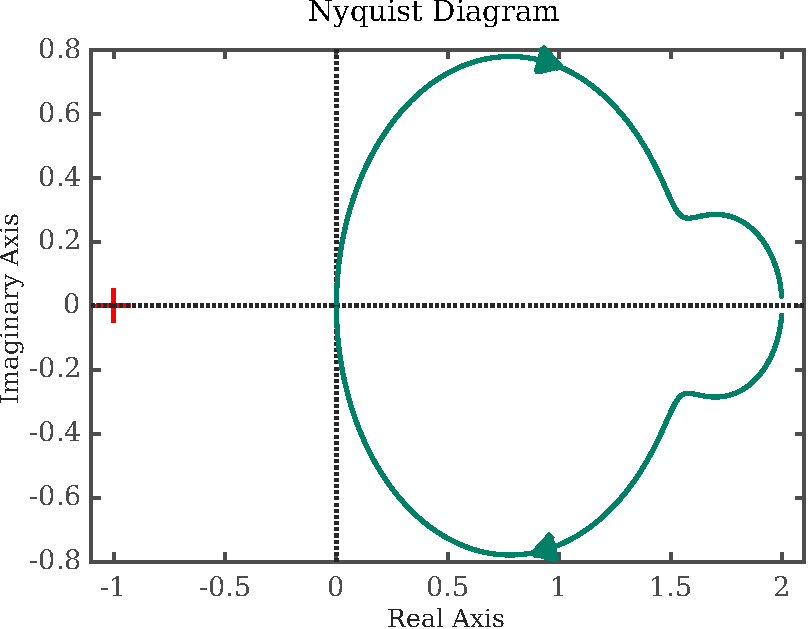
\includegraphics[width=\textwidth]{../images/task3/o1/GNA0.pdf}
			\caption{\(\tau = 0\)}
		\end{minipage}
		\hfill
		\begin{minipage}{\w}
			\centering
			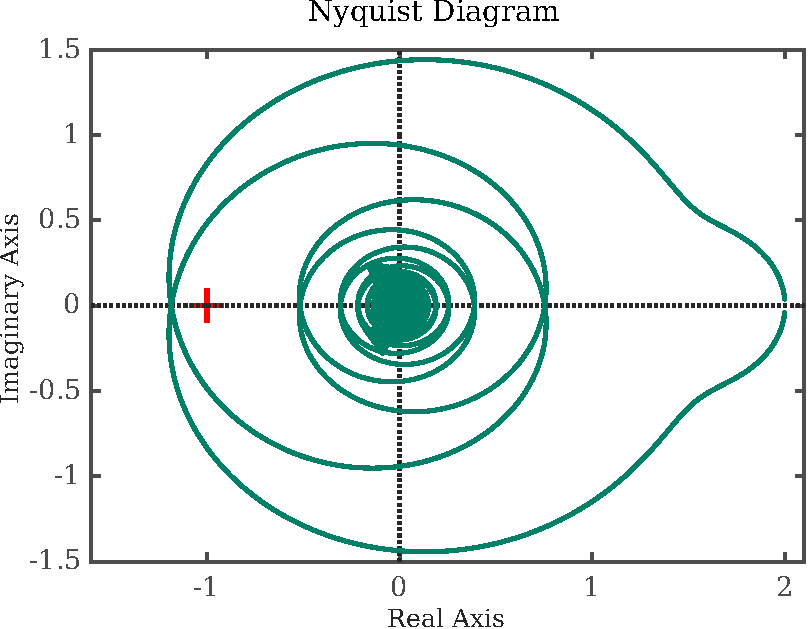
\includegraphics[width=\textwidth]{../images/task3/o1/GNA05.pdf}
			\caption{\(\tau = 0.5\)}
		\end{minipage}
		
		\caption*{Рисунки 45-46: Годографы Найквиста при \(\tau = 0\) и \(\tau = 0.5\)}
	\end{figure}	

	Также построю годографы при \(\tau = 0.2, \tau_{kr} = \dfrac{1}{3}, \tau = 0.7, \tau = 1.2\)
	
	\begin{figure}[H]
		\centering
		
		\newcommand{\w}{0.49\textwidth}
		
		\begin{minipage}{\w}
			\centering
			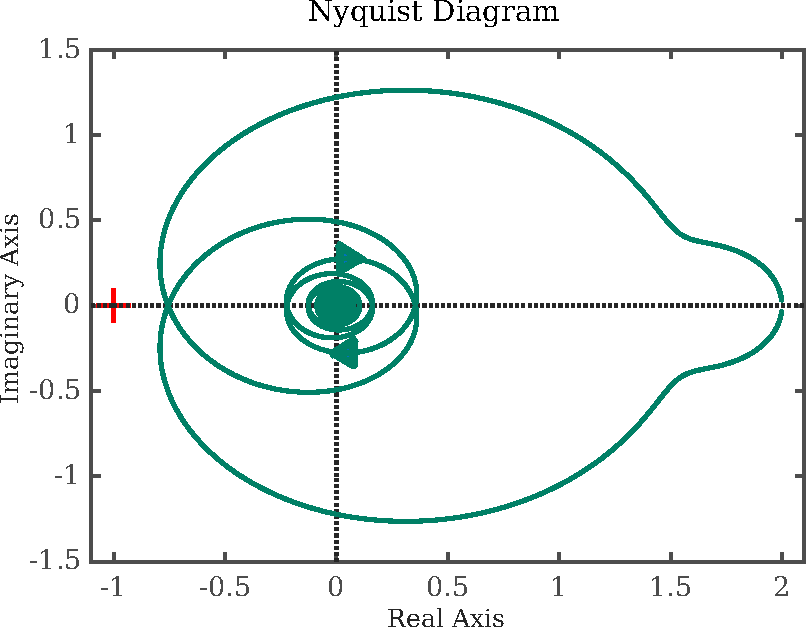
\includegraphics[width=\textwidth]{../images/task3/o1/GNA02.pdf}
			\caption{\(\tau = 0.2\)}
		\end{minipage}
		\begin{minipage}{\w}
			\centering
			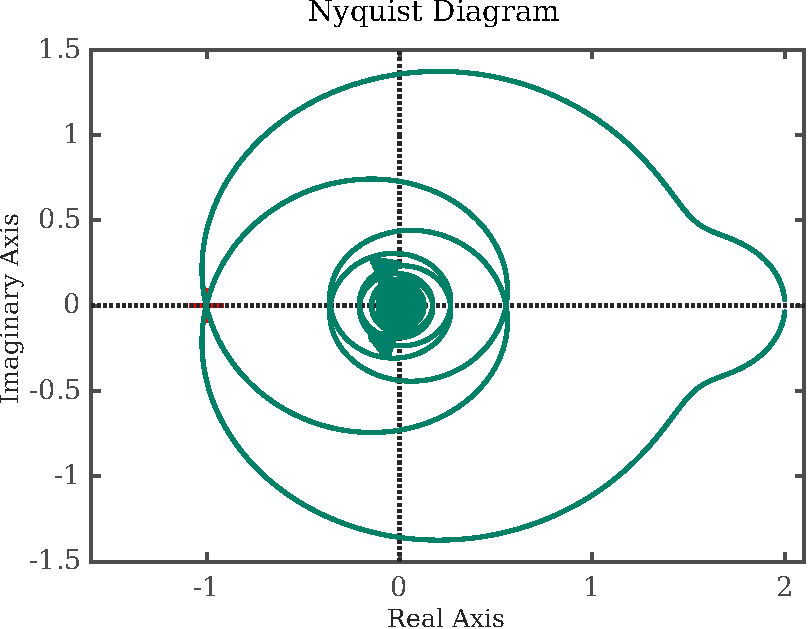
\includegraphics[width=\textwidth]{../images/task3/o1/GNA13.pdf}
			\caption{\(\tau = \dfrac{1}{3}\)}
		\end{minipage}
		
	\end{figure}	

	\begin{figure}[H]
		\centering
		
		\newcommand{\w}{0.49\textwidth}
		
		\begin{minipage}{\w}
			\centering
			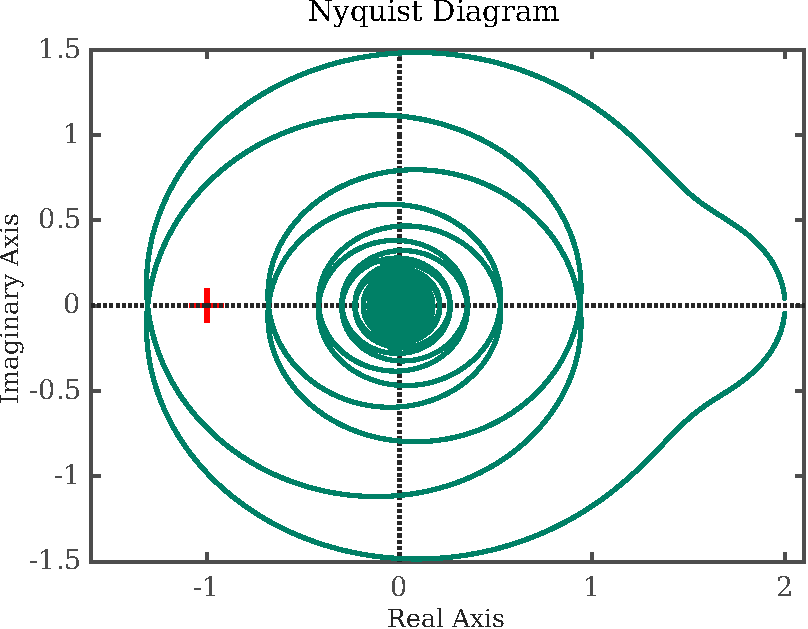
\includegraphics[width=\textwidth]{../images/task3/o1/GNA07.pdf}
			\caption{\(\tau = 0.7\)}
		\end{minipage}
		\begin{minipage}{\w}
			\centering
			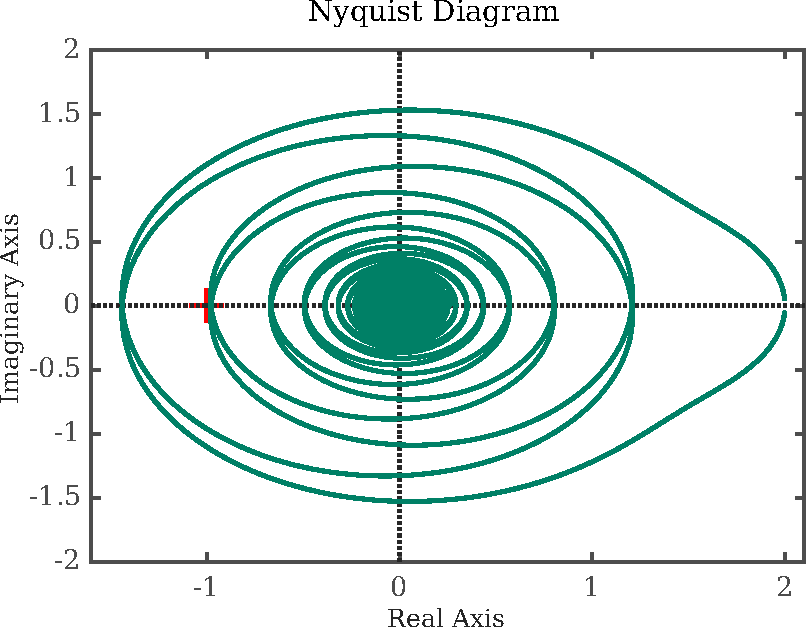
\includegraphics[width=\textwidth]{../images/task3/o1/GNA12.pdf}
			\caption{\(\tau = 1.2\)}
		\end{minipage}
		
		\caption*{Рисунки 47-50: Годографы Найквиста при различных \(\tau\)}
	\end{figure}	

	Получается, что при увеличении коэффициента запаздывания увеличивается количество оборотов годографа вокруг критической точки. Это влияет на устойчивость замкнутой системы -- чем больше оборотов \textit{по часовой} стрелке, тем больше неустойчивых полюсов будет у замкнутой системы. Также видно, что при \(\tau_{kr}\) линия годографа проходит через точку \((-1; 0)\), это означает, что замкнутая система будет находится на границе устойчивости. 

	\subsubsection{Переходные характеристики}
	
	Выберу значения коэффициента запаздывания для каждой из областей значений, соответствующих как устойчивой системе, так и неустойчивой:
	
	\[\tau_1 = \dfrac{1}{5} \qquad \tau_2 = \dfrac{1}{2} \qquad \]

	При \(\tau = \tau_1\) замкнутая система устойчива.
	
	При \(\tau = \tau_2\) замкнутая система неустойчива.
	
	\begin{figure}[H]
		\centering
		
		\newcommand{\w}{0.49\textwidth}
		
		\begin{minipage}{\w}
			\centering
			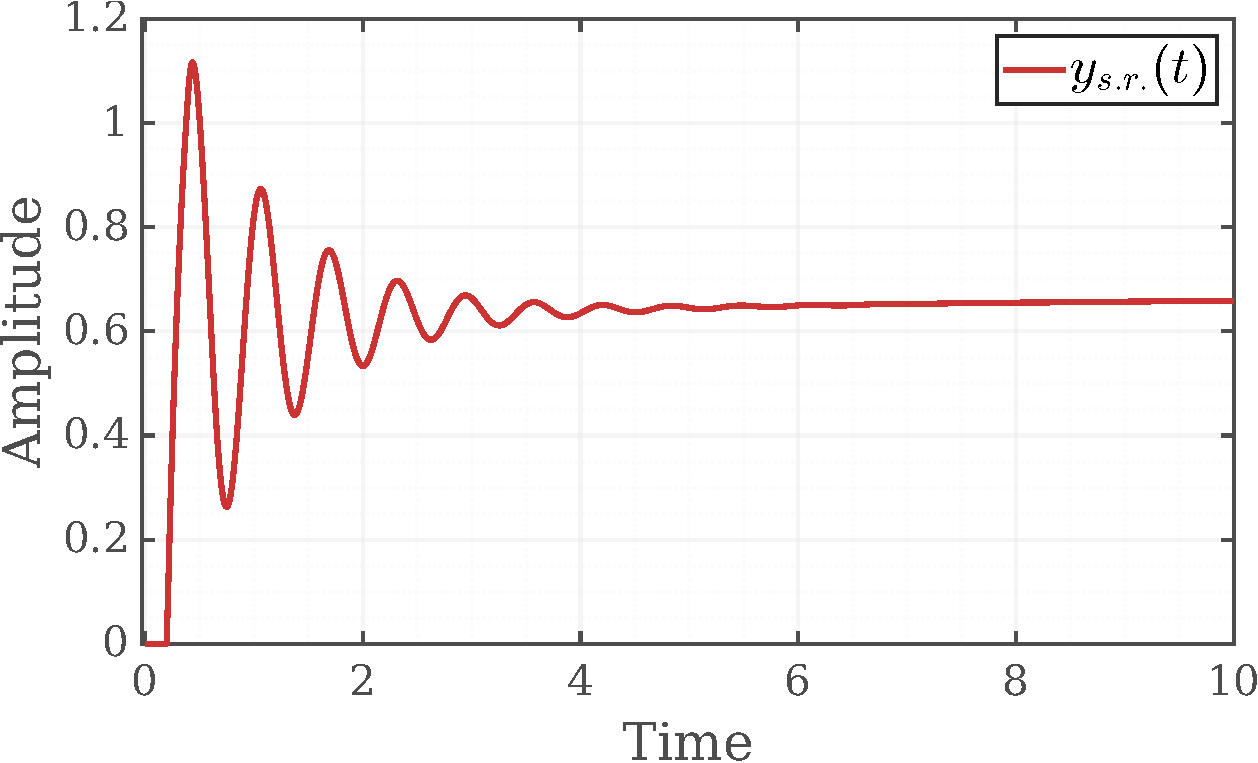
\includegraphics[width=\textwidth]{../images/task3/o1/h-zamk12.pdf}
			\caption{\(\tau = \dfrac{1}{5}\)}
		\end{minipage}
		\begin{minipage}{\w}
			\centering
			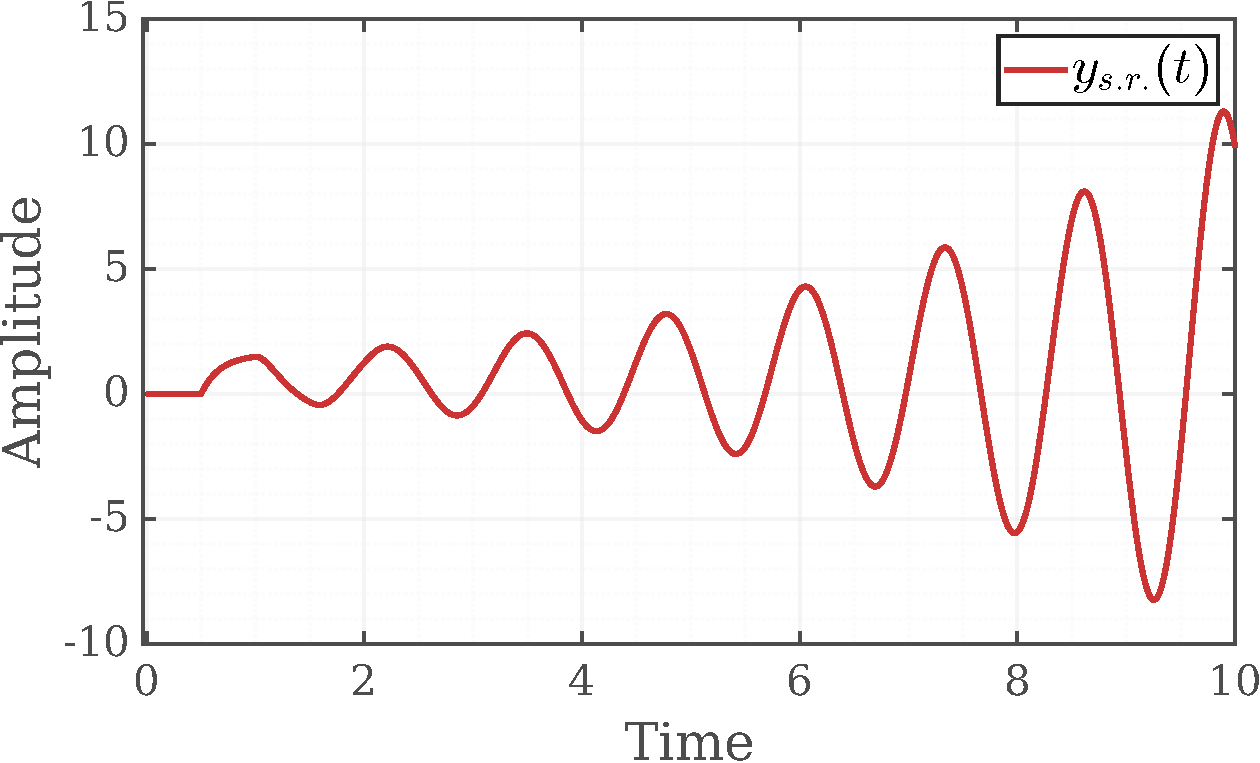
\includegraphics[width=\textwidth]{../images/task3/o1/h-zamk15.pdf}
			\caption{\(\tau = \dfrac{1}{2}\)}
		\end{minipage}
		
		\caption*{Рисунки 51-52: Step Response замкнутых систем для различных \(\tau\)}
	\end{figure}	



	\newpage
	\subsection{Объект 2}
	
	Второму объекту соответствует передаточная функция: \[W_4(s) = \dfrac{8s^2 + 4s + 2.4}{10s^2 - 5s + 11}\]
	
	Разомкнутая система имеет 2 неустойчивых полюса (дискриминант отрицательный, а вещественная часть положительна):
	
	\[n = 2\]
	
	Добавлю к объекту звено чистого запаздывания. Получится:  
	
	\[W(s) = \dfrac{8s^2 + 4s + 2.4}{10s^2 - 5s + 11} \cdot e^{-\tau s}\]
	
	\subsubsection{Расчёт критического \(\tau\) и запаса по фазе}
	
	Сначала проверю устойчивость замкнутой системы без запаздывания.
	
	Характеристическое уравнение замкнутой системы при \(\tau=0\):
	
	\[
	H(s) = 10s^2 -5s +11 + (8s^2 + 4s + 2.4) = 18s^2 - s + 13.4 = 0
	\]
	
	Корни:
	
	\[
	s = \frac{1 \pm j\sqrt{963.8}}{36}
	\]
	
	Так как действительная часть корней положительна, то замкнутая система неустойчива уже при \(\tau = 0\). Следовательно, исходная система \textit{не обладает} запасом устойчивости по фазе, так как при отсутствии запаздывания она уже является неустойчивой. 
	
	\medskip
	
	Посчитаю, критическое \(\tau\), при котором замкнутая система находится на границе устойчивости. Амплитуда и фаза объекта (при \(\tau = 0\)):
	
	\[W_4(s) = \dfrac{8s^2 + 4s + 2.4}{10s^2 - 5s + 11} \qquad W_4(j \omega) = \dfrac{ 8(j \omega)^2 + 4j \omega + 2.4}{ 10(j \omega)^2 -5j \omega + 11 } 
	= \dfrac{ (-8 \omega^2 + 2.4) +4j \omega}{ (-10 \omega^2 + 11) -5j \omega } \]
	
	\[A(\omega) = \dfrac{ \sqrt{(-8 \omega^2 + 2.4)^2 + (4 \omega)^2} }{ \sqrt{ (-10 \omega^2 + 11)^2 + (-5 \omega)^2 } } = 
	\dfrac{ \sqrt{ (-8 \omega^2 + 2.4)^2 + 16\omega^2 } }{ \sqrt{ (-10 \omega^2 + 11)^2 + 25\omega^2 } }\]
	
	
	\[\varphi(\omega) = \arctg \left(\dfrac{4\omega}{-8 \omega^2 + 2.4} \right) - \arctg \left(\dfrac{-5 \omega}{-10\omega^2 + 11} \right)\]
	
	Посчитаю значение частоты, при котором \(A(\omega) = 1\) и это будет \(\omega_{cp}\). Эта частота является частотой среза по усилению.
	
	\[	\dfrac{ \sqrt{ (-8 \omega_{cp}^2 + 2.4)^2 + 16\omega_{cp}^2 } }{ \sqrt{ (-10 \omega_{cp}^2 + 11)^2 + 25\omega_{cp}^2 } } = 1 
	\Longrightarrow \quad
	\omega_{cp}^2 =
	\frac{172.6 \pm \sqrt{13196.2}}{72}
	\Longrightarrow \quad
	\omega_{cp_{1,2}} \approx 0.895;\text{ } 1.998
	\]
	
	Таким образом, объект имеет две частоты среза по усилению.
	
	Для частот найду фазу и соответствующее критическое запаздывание:
	\[
	\varphi_{z}=\pi+\varphi(\omega_{cp}),
	\qquad
	\tau_{kr}=\frac{\varphi_{z}}{\omega_{cp}}
	\]
	
	Первая частота среза \(\omega_{cp_1} \approx 0.895\) рад/с:
	
	\[
	\varphi(\omega_{cp_1}) \approx -2.887
	\]
	\[
	\varphi_{z_1} = \pi + (-2.887) \approx 0.255
	\]
	\[
	\tau_{kr_1} = \frac{0.255}{0.895} \approx 0.284
	\]
	
	Вторая частота среза \(\omega_{cp_2} \approx 1.998\):
	
	\[
	\varphi(\omega_{cp_2}) \approx -0.597
	\]
	\[
	\varphi_{z_2} = \pi + (-0.597) \approx 2.545
	\]
	\[
	\tau_{kr_2} = \frac{2.545}{1.998} \approx 1.274
	\]
	
	Следовательно, частотам среза соответствуют два значения задержки:
	\[
	\tau_{kr_1} \approx 0.284 \text{ с} \qquad \tau_{kr_2} \approx 1.274 \text{ с}
	\]
	
	Тогда границы устойчивости:
	\begin{itemize}
		\item \(0 \leq \tau < \tau_{kr_1} \approx 0.284\) с~--- система неустойчива
		\item \(\tau_{kr_1} < \tau < \tau_{kr_2}\), \(0.284 < \tau < 1.274\) с~---
		система устойчива
		\item \(\tau > \tau_{kr_2} \approx 1.274\) с~--- система снова неустойчива
	\end{itemize}

	
	\newpage
	\subsubsection{Годографы Найквиста}
	
	Построю годографы Найквиста при отсутствии звена чистого запаздывания и при \(\tau = 0.5\). 
	
	При \(\tau = 0\) Годограф совершает 0 оборотов вокруг критической точки, а ранее я получила \(n = 2\), то по критерию Найквиста:
	
	\[n + X = m \quad \Longrightarrow \quad m = 2 + 0\]
	
	Значит замкнутая система имеет 2 неустойчивых полюса, значит она неустойчива.
	
	При \(\tau = 0.5\) Годограф совершает 2 оборота вокруг критической точки против часовой стрелки:
	
	\[n + X = m \quad \Longrightarrow \quad m = 2 + (-2) = 0\]
	
	Замкнутая система устойчива.
	
	
	\begin{figure}[H]
		\centering
		
		\newcommand{\w}{0.49\textwidth}
		
		\begin{minipage}{\w}
			\centering
			
\includegraphics[width=\textwidth]{../images/task3/o2/GNA0.pdf}
			\caption{\(\tau = 0\)}
		\end{minipage}
		\hfill
		\begin{minipage}{\w}
			\centering
			
\includegraphics[width=\textwidth]{../images/task3/o2/GNA05.pdf}
			\caption{\(\tau = 0.5\)}
		\end{minipage}
		
		\caption*{Рисунки 53-54: Годографы Найквиста при \(\tau = 0\) и \(\tau = 0.5\)}
	\end{figure}	
	
	Также построю годографы при \(\tau = 0.284, \tau_{kr} = 1.274\).
	
	В этих случаях годограф проходит через критическую точку, что означает границу устойчивости замкнутой системы.
	
	\begin{figure}[H]
		\centering
		
		\newcommand{\w}{0.49\textwidth}
		
		\begin{minipage}{\w}
			\centering
			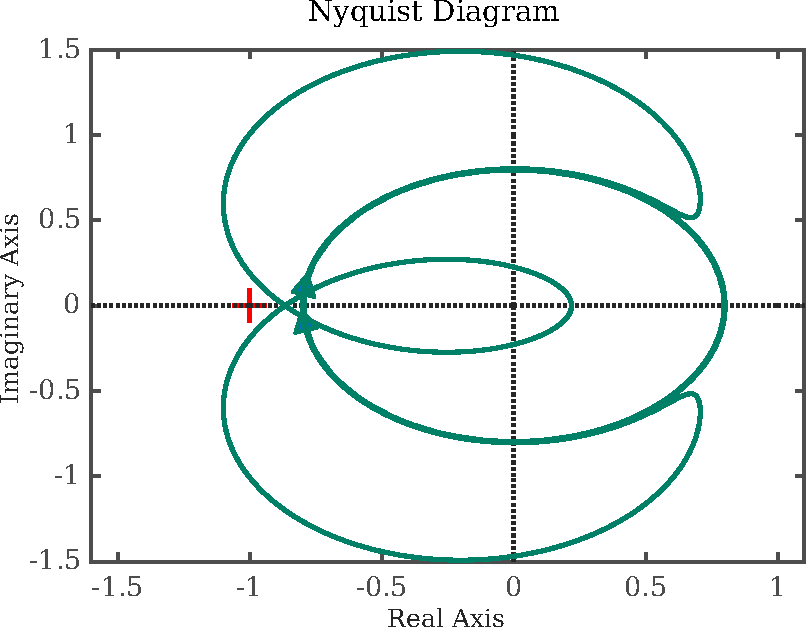
\includegraphics[width=\textwidth]{../images/task3/o2/GNA01.pdf}
			\caption{\(\tau = 0.284\)}
		\end{minipage}
		\begin{minipage}{\w}
			\centering
			
\includegraphics[width=\textwidth]{../images/task3/o2/GNA12.pdf}
			\caption{\(\tau = 1.274\)}
		\end{minipage}
		
		
		\caption*{Рисунки 55-56: Годографы Найквиста при различных \(\tau\)}
	\end{figure}	
	
	И наконец, годограф при \(\tau = 2\). В этом случае он не совершает обходов вокруг точки, замкнутая система не устойчива по критерию Найквиста.
	
	\begin{figure}[H]
		\centering
		
		\newcommand{\w}{0.5\textwidth}
		
		\begin{minipage}{\w}
			\centering
			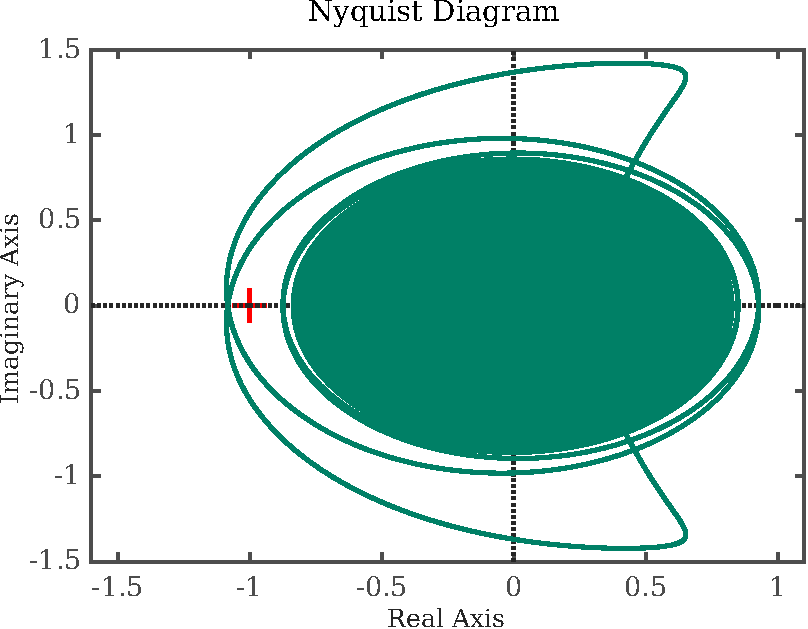
\includegraphics[width=\textwidth]{../images/task3/o2/GNA5.pdf}
			\caption{Годограф Найквиста при \(\tau = 2\)}
		\end{minipage}
		
	\end{figure}	

	Годографы Найквиста подтвердили предыдущий расчет.  Замкнутая система устойчива
	при \(0.284 < \tau < 1.274\), что соответствует двум обходам годографа против
	часовой стрелки вокруг точки \((-1;\,0)\), компенсирующим \(n = 2\) неустойчивых
	полюса разомкнутой системы:
	
	\[
	m({\tau}) =
	\begin{cases}
		2, & 0 \leq \tau < 0.284 \\
		0, & 0.284 < \tau < 1.274 \\
		2, & \tau > 1.274
	\end{cases}
	\]
	
	
	
	\subsubsection{Переходные характеристики}
	
	Выберу значения коэффициента запаздывания для каждой из областей значений,
	соответствующих как устойчивой системе, так и неустойчивой:
	\[
	\tau_1 = 1 \qquad \tau_2 = 2
	\]
	
	При \(\tau = \tau_1 = 1\) замкнутая система устойчива,
	так как \(\tau_1 \in (0.284;\, 1.274)\).
	
	При \(\tau = \tau_2 = 2\) замкнутая система неустойчива,
	так как \(\tau_2 > \tau_{kr_2} = 1.274\).
	
	\begin{figure}[H]
		\centering
		
		\newcommand{\w}{0.49\textwidth}
		
		\begin{minipage}{\w}
			\centering
			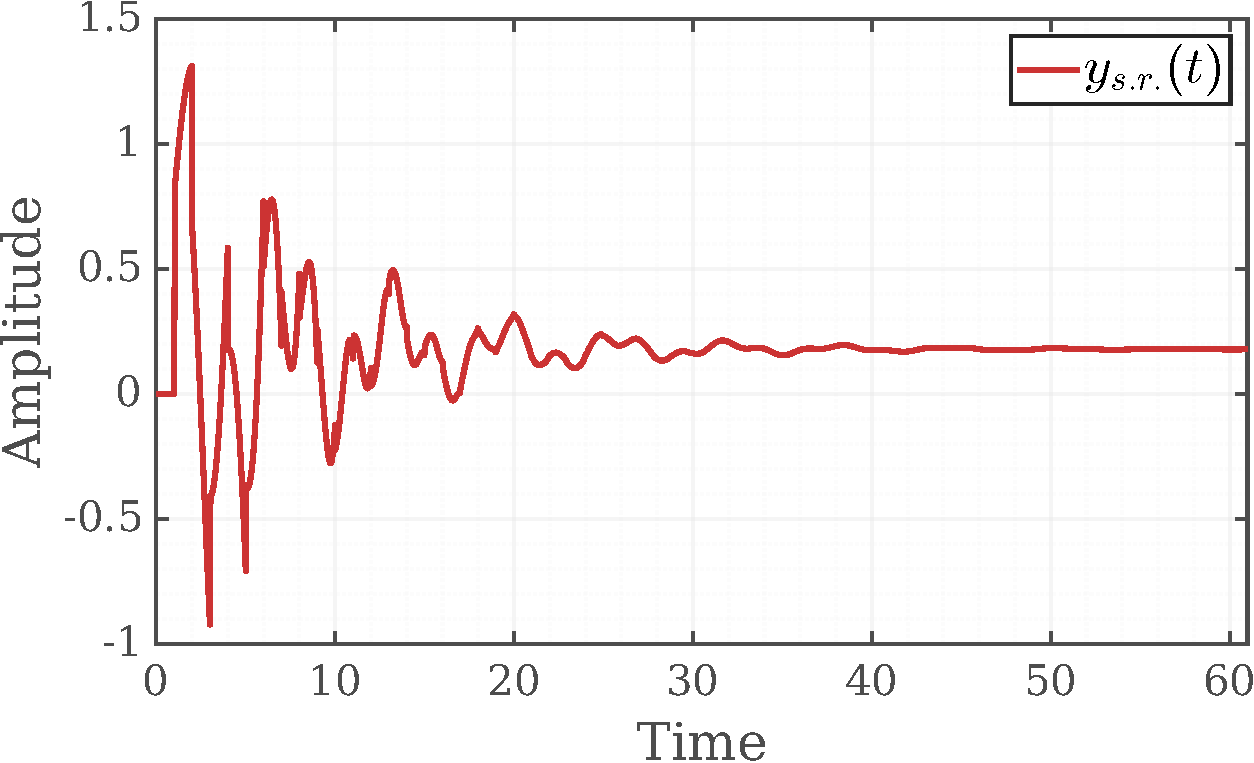
\includegraphics[width=\textwidth]{../images/task3/o2/h-zamk1.pdf}
			\caption{\(\tau = 1\)}
		\end{minipage}
		\begin{minipage}{\w}
			\centering
			
\includegraphics[width=\textwidth]{../images/task3/o2/h-zamk2.pdf}
			\caption{\(\tau = 2\)}
		\end{minipage}
		
		\caption*{Рисунки 58-59: Step Response замкнутых систем для различных \(\tau\)}
	\end{figure}	
	
	Таким образом, устойчивость наблюдается в диапазоне:
	\[
	0.284 < \tau < 1.274 
	\]
	
	\newpage
	\subsection{Вывод по заданию}
	В задаче я исследовала влияние звена чистого запаздывания на устойчивость
	двух замкнутых систем.
	
	Для первого объекта я установила, что система остаётся устойчивой при
	$\tau < 0.33$ и теряет устойчивость при увеличении запаздывания.
	
	Для второго объекта при $\tau = 0$ система неустойчива, однако введение
	запаздывания стабилизирует её. Устойчивость наблюдается в диапазоне
	$0.284 < \tau < 1.274$, при $\tau > 1.274$ устойчивость снова теряется.
	


	
	
	

	\newpage
	\section{Вывод}
	
	В лабораторной работе я исследовала устойчивость линейных систем с помощью критериев Найквиста, а также проанализировала влияние коэффициента усиления и звена чистого запаздывания. Полученные результаты показали согласованность всех методов и подтвердили, что изменение коэффициента усиления и времени 
	запаздывания существенно влияет на устойчивость замкнутой системы 
	и может как стабилизировать её, так и привести к появлению 
	неустойчивых полюсов.
	
	

	Материалы работы: \href{https://github.com/decadeos/ITMO/tree/master/3_course/lsau/lab6}{\texttt{github.com}}
	
	
	
	
\end{document}